\documentclass[galician]{./head/uvigo-tfg}
\usepackage{t1enc}
\usepackage[utf8]{inputenc}
\usepackage[galician]{babel}
\usepackage{amsmath,amssymb,amsthm}
\usepackage{algorithm}
\usepackage{algpseudocode}
\usepackage{changebar}
\usepackage[table]{xcolor}
\usepackage[marginratio=1:1,%
 paper=a4paper,tmargin=36pt,bmargin=3cm,lmargin=75pt,%
 includehead,twoside]{geometry}
\usepackage[pdftex,colorlinks=true]{hyperref}
\usepackage{./head/heading-uvigo} % Head of the UVigo
\usepackage[format=plain, labelfont=it, textfont=it, justification=centering, ]{caption}
\usepackage{graphicx}
\usepackage{subcaption}
\usepackage{cleveref}
%\title{Pedestrian Detection for low resources platforms}
\title{Detección de peóns para plataformas con baixos recursos}
\author{Ismael Orge Fernández}
\advisor{José Luis Alba Castro}
\academic{2019-2020}



\begin{document}
\begin{titlepage}

\Large
\sffamily

\begin{center}
  \begin{tabular}{c}
    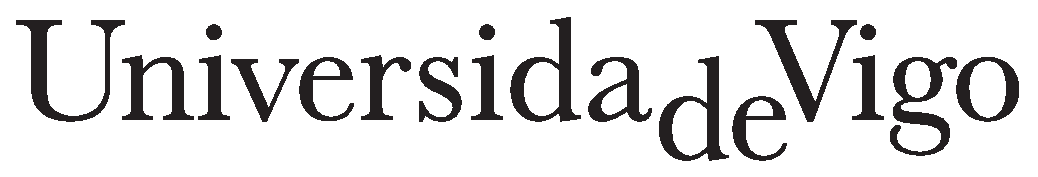
\includegraphics[width=0.55\textwidth]{./head/unilogo}
  \end{tabular}
\end{center}

\vfill
\begin{center}
  \huge DETECCIÓN DE PEÓNS PARA PLATAFORMAS CON BAIXOS RECURSOS
\vspace{26pt}\\
\textcolor{gray}{\small{}}
\end{center}

\vspace*{2cm}
\centerline{\huge 
Ismael Orge Fernández}

\vfill

\begin{center}
  \large
  Traballo de fin de grao \\
  Escola de Enxeñaría de Telecomunicación \\
 Grao en   Enxeñaría de Tecnoloxías de Telecomunicación
\end{center}

\vfill
\begin{center}
  Titor: \\
  José Luis Alba Castro\\
\end{center}
\vfill
\centerline{2019}
\end{titlepage}
\pagebreak
\pagebreak
\thispagestyle{empty}
\vspace*{12cm}



\begin{flushright}



\end{flushright}


\maketitle
\thispagestyle{plain} % To avoid head in all pages

%--------- INTRODUCIÓN ---------
    \section{Introdución}\label{intro}
    A detección de obxectos mediante a análise de imaxes reciviu unha gran atención nos últimos anos. A detección de peóns é un subtema moi popular nas últimas investigacións debido as súas diversas aplicacións, como pode ser o seguimento da súa traxectoria ou a predición desta mesma, extendéndonse a distintos campos: seguridade vial, videovixilancia, robótica... A pesar desta atención, o problema está lonxe de alcanzar un punto de saturación e os últimos estudos amosan avances significativos na fiabilidade das deteccións.
    \par Nos últimos anos, realizáronse diferentes aproximacións ao problema: \textit{HOG, SVM, Haar-like features, redes neurais...} Sendo as redes neurais (NN), en concreto as convolucionais (CNN), as máis investigadas na actualidade.
    Có auxe destas redes, probáronse novos métodos basados nelas e, aínda que ofrecen unha moi boa aproximación do problema, posúen unha gran desventaxa: a gran cantidade de información e operacións que hai que procesar e que leva á imposibilidade de poder utilizar equipos modestos (sen GPU dedicada por exemplo) para poder empregalas en tempo real.
    \par Neste traballo preténdese precisamente evitar esta necesidade mediante o uso de sistemas de procesado de imaxe tradicional (evitando as redes ou sistemas máis pesados) e a información a priori referente ao problema. Isto é, basándose en que, de forma xeral, pódese dicir que un peón aparece de pé nas imaxes podéndose empregar o seu contorno para caracterízalo\cite{zhang}. Tendo en conta que os detectores empregan grandes cantidades de características propias da imaxe para catalogala, isto permitirá utilizar características máis significativas en conxunto que se, por exemplo, se empregase un grupo de características xeradas aleatoriamente, como fan as redes.
    \par En definitiva, o obxectivo é chegar a un detector que utilice un mínimo de características o máis signifactivas posíbeis para poder disminuir a carga computacional.
    
%--------- OBXECTIVOS ---------
    \section{Obxectivos}
    Este proxecto enfócase principalmente na detección de peóns nunha posición ergueita nun entorno urbano mediante o emprego de \textit{Informed Haar-like Features}, proposto no paper de S. Zhang \cite{zhang}. Isto consiste en adestrar un algoritmo de aprendizaxe automática como clasificador cun determinado conxunto de datos. Neste caso estes datos foron imaxes de peóns.
    \par Para realizar este adestramento foi necesario facer:
     \begin{enumerate}
     \item \textbf{Procesado dos datasets}. Os datasets empregados non teñen unha imaxe por peón cun tamaño determinado se non que teñen distintas imaxes con varios peóns nelas. Por iso faise necesario un procesado dos dataset para separalos adecuademente e poder utilizalos no adestramento do detector, que necesita telos claramente separados e nun tamaño predeterminado.
     
     \item \textbf{Xeración dos templates e cálculo das características}. Xerar templates rectangulares en base o xa comentado do contorno do peón e evitando a información redundante así como calcular as características das imaxes a empregar nos adestramentos.
     
     \item \textbf{Selección e adestramento dos detectores}. É o punto máis crítico xa que supón precisar que modelos se van a empregar na detección e con qué parámetros, o que terá unha forte influencia no resultado final.
     \item \textbf{Comparativa entre os distintos detectores adestrados}. Unha comparativa entre os detectores adestrados na que se mostran resultados como o tempo de procesado ou a precisión do clasificador.
     \end{enumerate}
     
%--------- DESENVOLVEMENTO --------- 
    \section{Desenvolvemento}
    Nesta sección descríbese a metodoloxía seguida e as decisións técnicas tomadas para a implementación deste proxecto. Para elo, o proceso realizado desglósase nos seguintes puntos:
    \begin{enumerate}
        \item \textbf{Procesado dos datasets}. Como se empregaron os datasets e que cambios foron necesarios nos datos.
        \item \textbf{Extracción da imaxe media de contornos dun peón}. Como se obtivo o mapa de contornos e qué se fixo logo con el.
        \item \textbf{Xeración dos templates}. Qué son os templates e como se xeraron para este proxecto.
        \item \textbf{Cálculo das características}. Cómo se obtiveron as características para alimentar os clasficadores e cómo son neste caso.
        \item \textbf{Adestramento do clasificador} Qué tipo de adestramento se seguiu, e explicación do clasificador que se empregou nel.
    \end{enumerate}
     \par Os puntos están ordeados para seguir o proceso de forma lóxica e conteñen as definicións dos termos necesarios para o seu entendemento.
    \par Este proxecto está completamente feito en Python empregando os módulos scikit-learn\cite{scikit-learn} e CatBoost\cite{CatBoost} para os clasificadores e os datasets de INRIA\cite{inria} e Caltech\cite{caltech} para os adestramentos.
      %--------- DATASETS ---------
        \subsection{Procesado dos datasets}\label{datasets} Ámbolos datasets (INRIA e Caltech) proporcionan un conxunto de imaxes nas que se poden encontrar peóns xunto cunhas anotacións nas que se localiza en cada imaxe a súa posición é tamaño.
        \par Para realizar o adestramento foi necesario ter un conxunto con imaxes positivas (aquelas que conteñen peóns na imaxe) e outro con imaxes negativas (aquelas que non conteñen peóns). Non obstante a diferencia entre os formatos das anotacións e das imaxes fixo que houbese que tratar cada dataset por separado para extraer os datos que se ían utilizar. 
        \par No caso de Caltech,  foi necesario extraer as imaxes das secuencias de video e as anotacións dun ficheiro con formato de Matlab a un JSON debido a que estes datos  non era facilmente procesábeis en Python có formato orixinal. Tanto para a extracción coma para o formato utilizouse o extractor facilitado por Saito Shunta para este dataset\cite{Saito}. En canto ás imaxes negativas, tivéronse que extraer aleatoriamente das imaxes principais evitando que contivesen algún fragmento de persoa, xa que este dataset non adxunta un set de negativos.
        \par  No caso de INRIA, o dataset xa viu coas imaxes separadas en positivas e negativas e coas anotacións nun formato .txt, polo que non foi necesario facer ningunha conversión. Ademais, este dataset, ao contrario que Caltech, si contén un set de imaxes negativas.
        \par Unha vez obtidos os dous conxuntos de imaxes, recortáronse a un tamaño dado para adestrar logo o clasificador, tendo en conta que no caso dos positivos os peóns aparecen centrados na imaxe e cun certo marxe por cada lado.
        \par Para os dous datasets as imaxes finais recortadas para o adestramento do clasificador foron de 60x120 píxels cómo propón S. Zhang\cite{zhang}\cite{alarcon} tanto para as positivas coma para as negativas. Desta maneira tivéronse dous sets de imaxes:
         \begin{enumerate}
            \item Set de adestramento Caltech: Que consistiu en 24596 imaxes de adestramento (4360 positivos + 20236 negativos) e 25275 imaxes de testeo (3119 positivos e 22156 negativos).
            
            \item Set de adestramento INRIA: Que consistiu en 23435 imaxes de adestramento (3407 positivos + 20028 negativos) e 13091 imaxes de testeo (3069 positivos + 10022 negativos).
        \end{enumerate}
  
        
    %--------- MAPA DE CONTORNOS ---------
    \begin{figure}[t]
        \centering
        \begin{subfigure}{.5\textwidth}
          \centering
          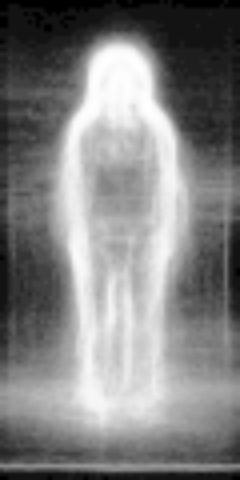
\includegraphics[width=.4\linewidth]{figures/edge_map_resized.png}
          \caption{Mapa medio de contornos dun peón}
          \label{fig:average1}
        \end{subfigure}%
        \begin{subfigure}{.5\textwidth}
          \centering
          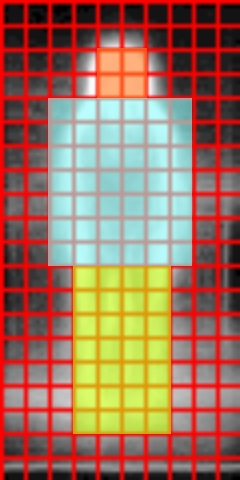
\includegraphics[width=.4\linewidth]{figures/edge_map_grid.png}
          \caption{Mapa de contornos coas zonas de interese xa segmentadas}
          \label{fig:average2}
        \end{subfigure}
        \caption{En (a) pódese observar o mapa obtido a partir do operador Canny mentres que en (b) vése a segmentación en cabeza(laranxa), torso(azul) e pernas(amarelo).  }
        \label{fig:averageEdgeMap}
    \end{figure}
        \subsection{Extracción da imaxe media de contornos dun peón} Para obter información sobre a forma dos peóns, realizouse unha detección de bordes sobre tódalas imaxes positivas, facendo logo un mapa promedio destes bordes. Para a detección empregouse a función Canny\cite{canny1987computational} da libraría OpenCV\cite{opencv_library}.
        \par A partir deste mapa, poidéronse etiquetar, delimitando as zonas dunha forma visual, tres partes diferenciadas: \textit{cabeza, torso e pernas} (Fig. \ref{fig:average1}).
        \par Unha vez feito isto, dividiuse a imaxe nunha malla de celdas de 6x6 píxels (dimensións que presentan un mellor funcionamento \cite{zhang}), clasificando cada celda manualmente como unhas das posíbeis opcións dependendo de cal destas zonas teña unha maior cobertura nesa celda: cabeza, torso, pernas ou fondo (Fig. \ref{fig:average2}).
        
    %--------- TEMPLATES ---------
        \subsection{Xeración dos templates}\label{templ}
        Os clasificadores, como son AdaBoost e CatBoost, necesitan como entrada unha serie de características que se calculan a partir de información extraída da imaxe (cor, magnitude do gradiente...). Non obstante, non é necesario utilizar a completitude desta información, senón que se pode seleccionar certos patróns que se repitan ao longo desta, evitando así, en parte, información redundante e reducindo a cantidade de datos. Estes patróns son os que reciben o nome de \textit{templates}.
        \par Entón, para conseguir os \textit{templates} tense que: coa malla de celdas xa debidamente etiquetada, xeráronse tódalas posíbeis combinacións de etiquetas en matrices dende dimensións 2x1 ata 4x4 e pasáronse ao longo da malla, escollendo como candidatas para o seguinte paso aquelas que coincidisen os seus valores no mapa (sen ter en conta matrices que teñan o mesmo valor en tódolos seus elementos). Estas matrices selecciondas son os \textit{templates} e foron empregadas logo no cálculo das características. 
        \par Indo un pouco máis en profundidade na xeración destas matrices: Primeiro, definíronse un conxunto de tamaños tal que
        \begin{equation}
            S = \{(w,h) \mid w \leq w_m, h \leq h_m,w,h \in \mathbb N^+\},
        \end{equation}
        onde $w$ e $h$ indican ancho e alto en termos de celdas para un \textit{template} e $w_m$ e $h_w$ o tamaño máximo destes \textit{templates} que neste caso poden ir dende 2x1 ata 4x4 celdas.
        \par A cada un dos \textit{templates} presentes asígnaselle un conxunto de etiquetas $L$ tal que para cada celda $c(i,j)$ existe unha etiqueta $L(i,j)$ que indica o compoñente presente nesa celda. 
        \par Logo, para cada par de dimensións $S$, deslízase unha xanela (\textit{sliding window}) ao longo de toda a imaxe do mapa de contornos para xerar \textit{templates} en diferentes posicións e con diferentes pesos. Para unha posición $(x,y)$ o \textit{template} xerado dependerá de cantas partes diferentes conteña. Cando sólo haia dúas xerarase un \textit{template} binario e cando haia tres, un ternario (Fig. \ref{fig:templates}).
        \par O conxunto de \textit{templates} resultante sería
        \begin{equation}
            T = \{(x,y,s,W) \mid x,y\in \mathbb N , s \in S,W \in \mathbb R^2\},
        \end{equation}
        onde $x$ e $y$ indican a posición do \textit{template} (en celdas), $s$ as dimensións do template e $W$ unha matriz de pesos determinada en base ao conxunto de etiquetas $L$ (Fig. \ref{fig:templates}). Un exemplo de matriz $W$ sería para un caso dunha matriz 3x1:
        \begin{equation}
            W=(-1,-1,1)
        \end{equation} 
        onde poderíase corresponder a etiqueta -1 a torso e 1 a pernas.
        \begin{figure}
            \centering
            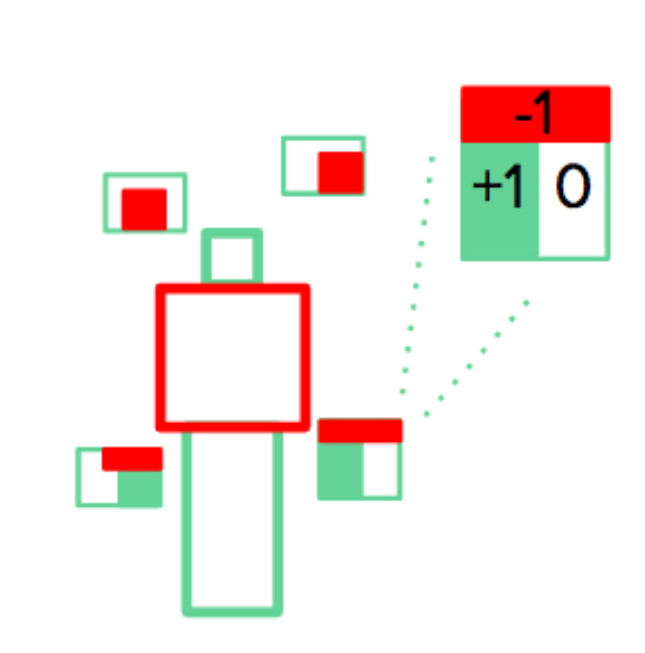
\includegraphics[height=200px]{figures/templates_gen.png}
            \caption{Exemplo de posíbeis templates xerados a partir da forma extraída do mapa de contornos}
            \label{fig:templates}
        \end{figure}
        \par Como neste caso pode haber \textit{templates} ternarios (pode haber zonas nas que apareza torso, pernas e fondo ou cabeza, torso e fondo), o etiquetado tradicional dos pesos como $+1$ e $-1$ para empregar en $W$ non é suficiente,  polo que se optou por utilizar no caso dos ternarios o conxunto $\{-1,0,+1\}$ (Fig. \ref{fig:templates}) mentres que nos binarios usouse $\{-1,+1\}$. O valor 0 no caso dos \textit{templates} ternarios reservouse sempre para o fondo.
        \par En total, e collendo unicamente aqueles \textit{templates} que son distintos entre sí e non \textit{templates} có mesmo valor en tódolos seus elementos, obtivéronse uns \textbf{1047 templates distintos} a partir do mapa de contornos. Estes \textit{templates} son os que logo usáronse no seguinte punto para o cálculo de características que se empregaron como entrada dos clasificadores.
        
    %--------- CARACTERÍSTICAS ---------
        \subsection{Cálculo das características} Unha vez obtidos os \textit{templates}, para extraer as carecterísticas dunha imaxe foi necesario ter distintos tipos de información dela sobre os que empregar estes \textit{templates}. En base a outras investigacións \cite{dollar2009integral}\cite{zhang}\cite{filtered}, HOG (Histogram of Oriented Gradients) é un dos máis informativos para este tipo de traballos así coma información sobre a cor presente na imaxe. Tamén é comunmente utilizada a información sobre magnitude do gradiente \cite{alarcon}.
        \par Para empregar tanto a información de cor coma a de gradiente, as características son multi-canal, isto é, para cada \textit{template} temos unha característica por canal, onde cada un deles é un tipo distinto de información. Elíxense así 10 canais:\textbf{ 3 canais de cor no espazo LUV, 1 canal con información de magnitude de gradiente e 6 canais para HOG}. Desta forma, para cada template tivéronse 10 valores distintos, un por cada canal.
        \par Entón, para calcular as características correspondentes a un \textit{template} tense que:
        \par Dado un \textit{template} $t=(x,y,(w,h),W)$ poderíase calcular a matriz de pesos media como
        \begin{equation}
            W_{avg}=\frac{sgn(W)}{n_{add}} + \frac{sgn(-W)}{n_{sub}},
        \end{equation}
        onde  $n_{add}$ é a cantidade de pesos $+1$ presentes no \textit{template} e $n_{sub}$ a cantidade de $-1$ (de ahí a elección do conxunto $\{-1,+1\}$ para os templates binarios). Utilizando esta matriz $W_{avg}$ poderíase calcular o valor dunha característica $f$ para un \textit{template} $t$ e un canal $k$ tal que
        \begin{equation}
            f(t,k)=\sum_{i=1}^h \sum_{j=1}^w \sigma(x+i,y+j,k)W_{avg}(i,j),
        \end{equation}
        onde $\sigma(i,j,k)$ define a suma de todos os valores nas celdas $c(i,j)$ para o canal $k$.
        \par Tendo en conta que por cada canal hai uns 1047 \textit{templates}, por cada imaxe existen unhas $1047 \times 10=10470$ características.
        \par Estas características son as que logo se empregaron como entrada para o adestramento do clasificador. Unha vez adestrado, a partir destas características, calculadas para unha imaxe, será capaz de determinar se existe un peón ou non.

        
    %--------- adestramento ---------
        \subsection{Adestramento do clasificador}\label{training} Para o adestramento empregouse o clasificador AdaBoost presente no módulo scikit-learn\cite{scikit-learn} de Python en ámbolos datasets (INRIA e Caltech). Ademais tamén utilizouse o clasificador CatBoost\cite{CatBoost} por dar bos resultados nas últimas investigacións e  permitir realizar o adestramento en GPU \cite{CatBoost}.
       \begin{figure}[t]
            \centering
            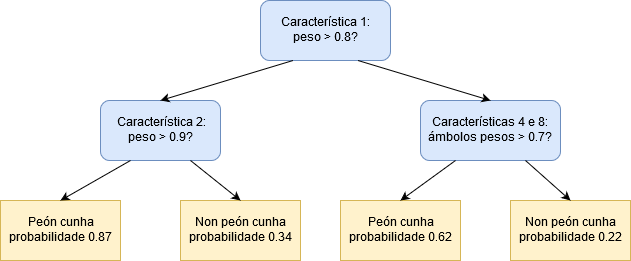
\includegraphics[height=150px]{figures/DecisionTreeExample.png}
            \caption{Exemplo dunha posíbel árbore de decisión resultante do adestramento do clasificador.}
            \label{fig:decisionTree}
        \end{figure}
        \par Ámbolos clasificadores (AdaBoost e CatBoost) son meta-algoritmos de aprendizaxe automática que se empregan en conxunto con outros algoritmos para mellorar os resultados. A saída final é unha suma ponderada da combinación da saída dos outros algoritmos (\textit{weak learners}). Para estes \textit{weak learners} escolleuse neste caso o algoritmo de árbores de decisión. Tamén empregouse o parámetro \textit{learning rate} que nestes clasificadores trátase dun valor que controla canto cambia o modelo en resposta ao erro estimado cada vez que se recalculan os pesos dos \textit{weak leaerners}.
        \par Para tódolos casos utilizouse un adestramento multironda consistente nun adestramento inicial do clasificador que logo é seguido dunha ronda de readestramento. A pesar do recomendado para os mellores resultados (3-4 rondas)\cite{zhang}\cite{filtered}, neste caso elexiuse unicamente de 2 rondas por mor do tempo (o caso de 4 rondas prolongaba o adestramento arredor dunha semana mentres que en 2 rondas quedouse en 2 días). Este foi levado a cabo nun PC cun procesador i7-6850K@3.6GHz, 32Gb de RAM e dúas NVIDIA 1080 GTX 12Gb GPU.
        \par As rondas consistiron en:
        \begin{enumerate}
            \item Ronda inicial: O clasificador iniciouse cunhas 1024 árbores de decisión de profundidade 2 (exemplo na Fig. \ref{fig:decisionTree}) e $0.001$ de learning rate no caso de AdaBoost e $0.01$ no caso de CatBoost. Para esta ronda empregouse todo o set de adestramento (sección \ref{datasets}).
            \item Ronda de readestramento: Unha vez rematada a ronda inicial, obteuse un clasificador funcional que logo se mellorou mediante unha segunda ronda de adestramento. Para esta ronda empregáronse os chamados negativos fortes: aquelas imaxes que, sendo negativas, o clasificador identifica coma positivas. Este tipo de imaxes son máis significativas para o adestramento, xa que supoñen os casos onde o algoritmo adestrado erra na súa clasificación.
            \par Para obter estes negativos fortes implementouse un \textbf{detector} que segue os seguintes pasos:
            \begin{enumerate}
                \item \textbf{Extracción de subimaxes}. A partir da imaxe principal que se lle pasa, o detector reescala a imaxe mediante un factor de escala tantas veces como poda ata que a imaxe sexa igual ou máis pequena que a xanela empregada no adestramento (60x120 píxels). A partir de cada unha destas imaxes reescaladas, extráense todas as subimaxes posíbeis de tamaño 60x120 empregando unha xanela deslizante para recortalas.
                \item \textbf{Cálculo dos canais}. Para cada subimaxe obtida, calcúlanse os 10 canais que se van a empregar para a extracción das características (3 canais de cor no espazo LUV, 1 canal con información de magnitude de gradiente e 6 canais para HOG).
                \item \textbf{Cálculo das características}. Empregando os templates (sección \ref{templ}) e os canais extraidos da subimaxe, o detector calcula as características.
                \item \textbf{Clasificación da imaxe}. Coas caraterísticas calculadas, o detector alimenta ao clasificador e este devólvelle a probabilidade de que a imaxe sexa un peón ($probabilidade>0.5$).
            \end{enumerate}
            
            \par Polo tanto, aquelas subimaxes que deron como positivas en imaxes negativas, son as que se poideron clasificar como negativos fortes. Unha vez obtidos al menos uns 10000 destes negativos, engadíronse ao set de entranamento e volveuse a adestrar o clasificador. Para esta ronda, ademais, cambiouse o número de árbores a 2048 de profundidade 2\cite{filtered}.
        \end{enumerate}
        \begin{figure}[t]
            \centering
            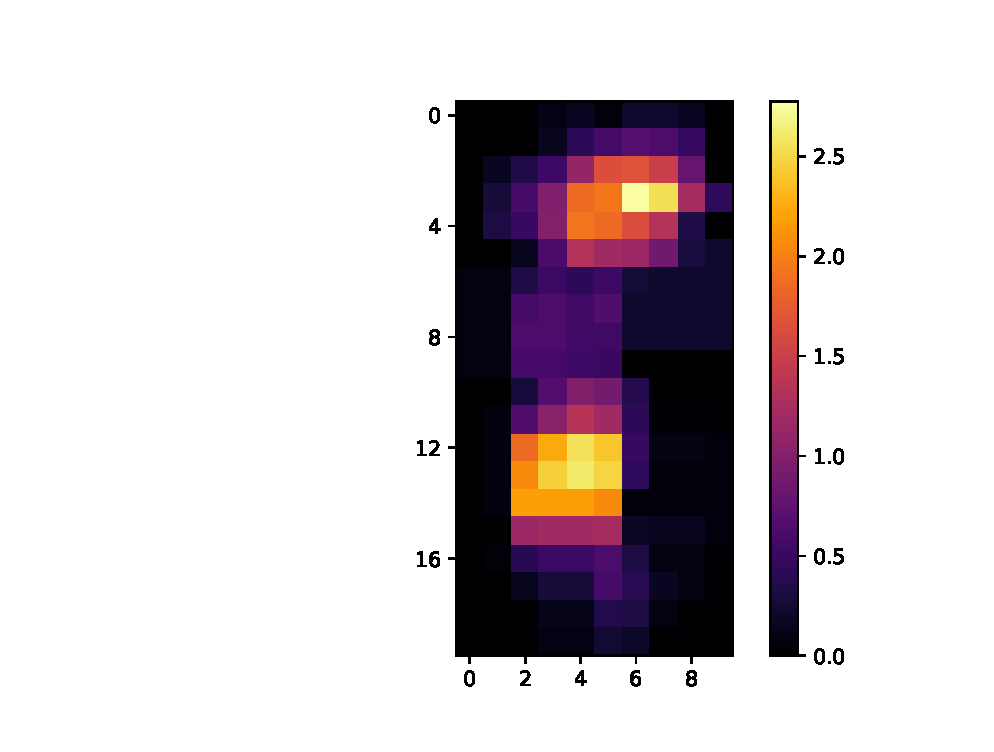
\includegraphics[height=200px]{figures/color_map.eps}
            \caption{Mapa de pesos das características: Pódese observar como as características máis importantes atópanse principalmente na cabeza e no cambio de torso a pernas. Esta imaxe foi extraída empregando o clasificador CatBoost adestrado para o dataset INRIA e a cor varía en función do peso acumulado en cada celda.}
            \label{fig:colormap}
        \end{figure}
        \par Os resultados proxectados por cada dataset diverxen bastante entre si, xa que Catech é considerado un dataset moito máis esixente ca INRIA, que aínda sendo un dos máis coñecidos e empregados, é máis pequeno e menos desafiante.
        \par Para facer unha mostra daquelas características máis significativas, na Fig. \ref{fig:colormap} amósanse as 100 primeiras características que tiveron un maior peso(importancia) no adestramento.
    

%--------- RESULTADOS ---------
    \section{Resultados}
    \par Unha vez adestrados os clasificadores, estes utilizáronse sobre as imaxes de testeo previamente saparadas das utilizadas para o adestramento (sección \ref{datasets}). Os resultados obtidos clasifícanse en tres tipos: peóns detectados correctamente, peóns non detectados e peóns que foron detectados incorrectamente (non aparecen na imaxe).
    Con estes resultados, pódense empregar as seguintes métricas para medir a efectividade dos clasificadores\cite{metrics}:
    \begin{enumerate}
        \item Detection rate (DR): Porcentaxe de deteccións correctas sobre tódolos peóns que poden ser detectados.
        \begin{equation}
            DR=\dfrac{DP}{NP} \times 100 \%,
        \end{equation}
        Onde $DP$ é o número de peóns detectados correctamente e $NP$ o número total de peóns detectábeis.
        \item False detection rate (FR): Porcentaxe de falsas deteccións sobre tódolos peóns que poden ser detectados. Unha falsa detección considérase cando detecta un obxecto pero este non é un peón.
        \begin{equation}
            FR = \dfrac{FP}{NP} \times 100 \%
        \end{equation}
        Onde $FP$ é o número de obxectos detectados erroneamente coma peóns.
        \item Missing rate (MR): Porcentaxe de peóns que non foron detectados sobre tódolos posíbeis peóns detectábeis.
        \begin{equation}
            MR = \dfrac{NP - DP}{NP} \times 100 \%
        \end{equation}
    \end{enumerate}
    \begin{figure}
        \centering
        \begin{subfigure}{.475\textwidth}
          \centering
            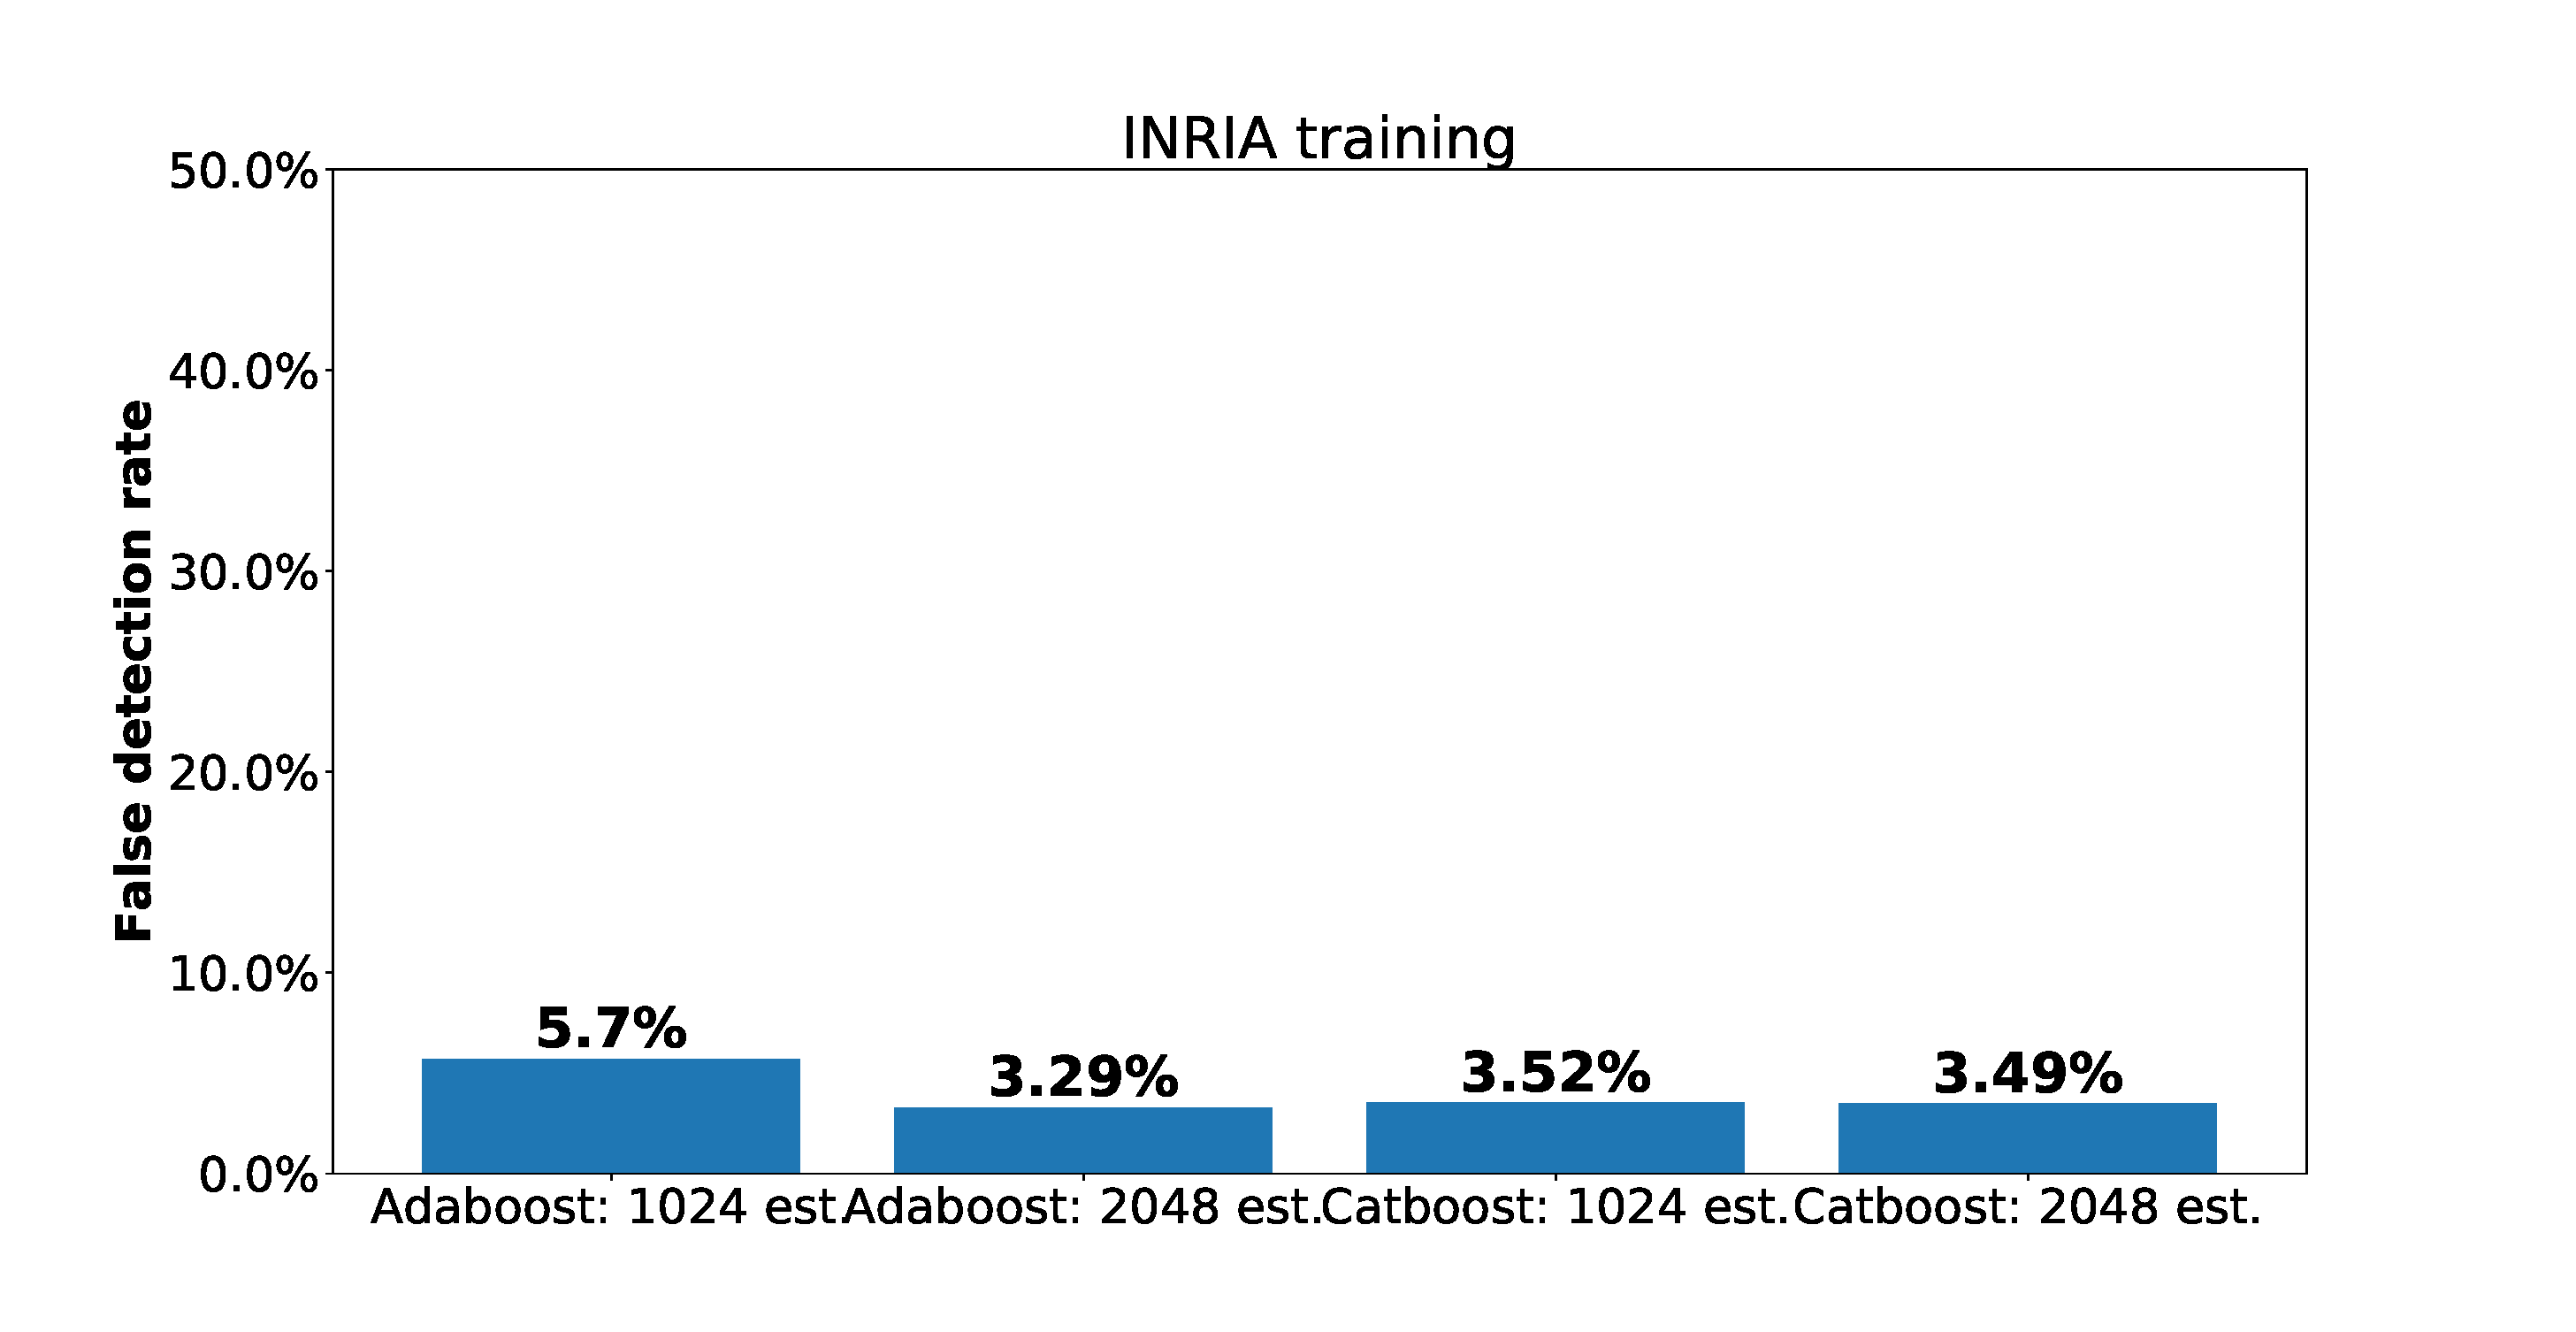
\includegraphics[width=1.1\linewidth]{figures/inria_false_detection.eps}
          \caption{False detection rate para os clasificadores AdaBoost e CatBoost.}
          \label{fig:sub1}
        \end{subfigure}%
        \begin{subfigure}{.475\textwidth}
          \centering
          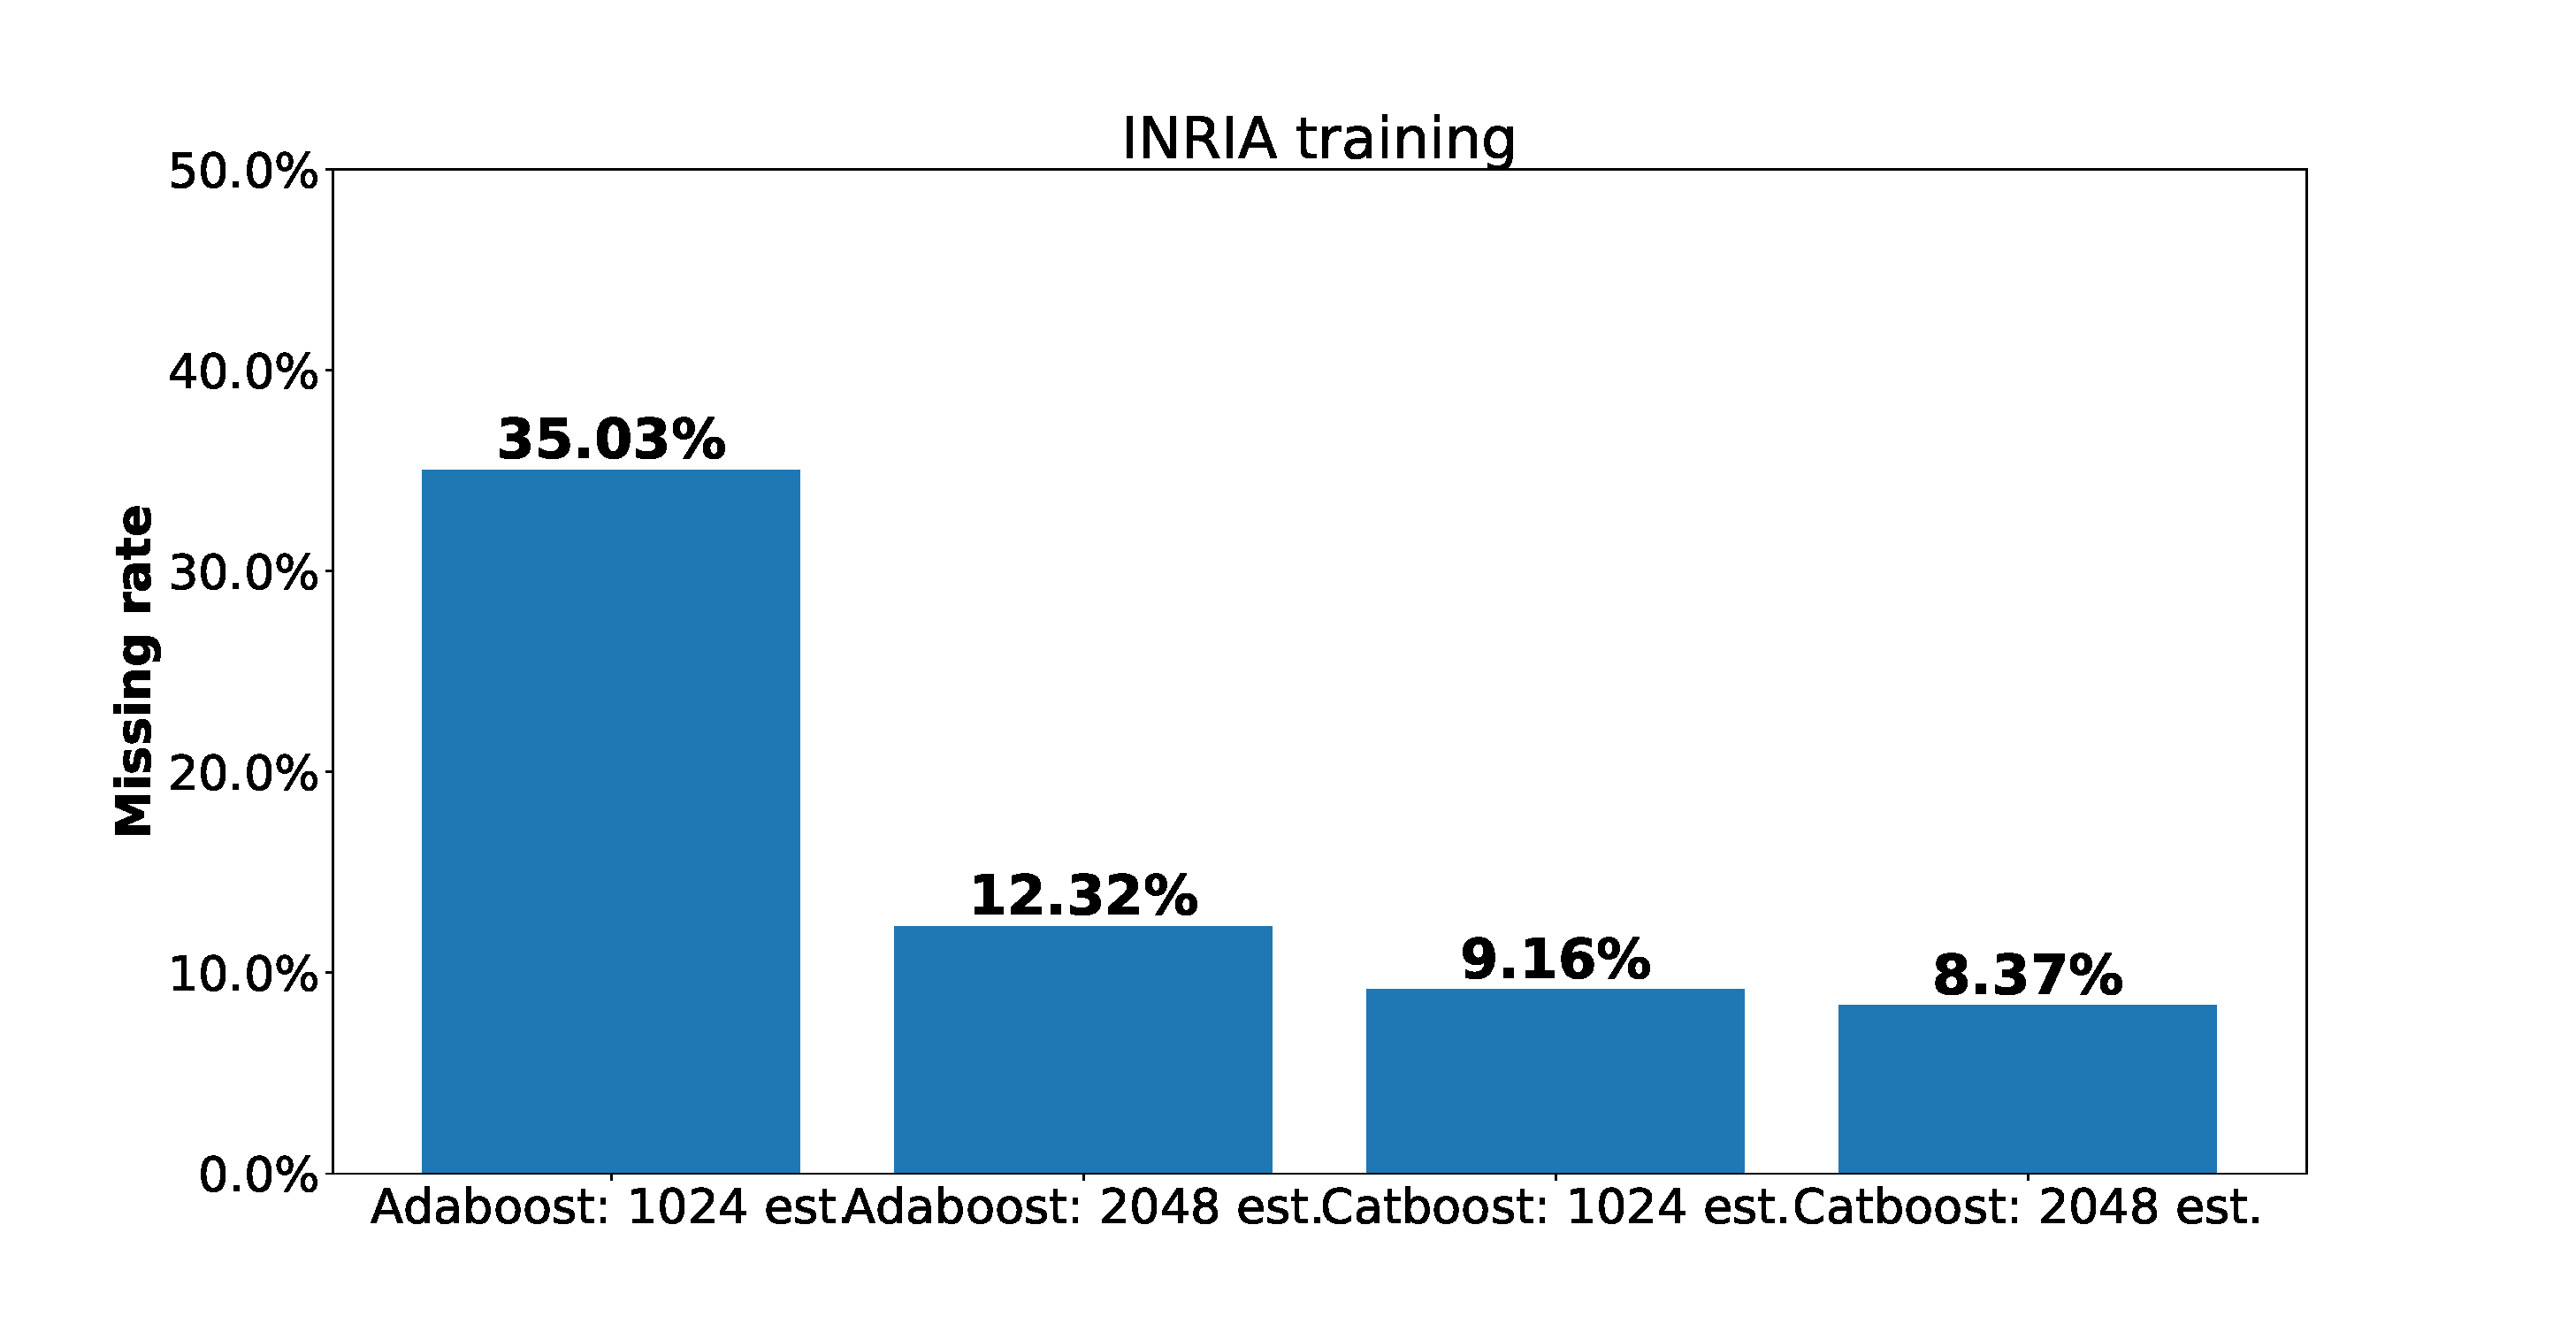
\includegraphics[width=1.1\linewidth]{figures/inria_missing_rate.eps}
          \caption{Missing rate para os clasificadores AdaBoost e CatBoost}
          \label{fig:sub2}
        \end{subfigure}
        \begin{subfigure}{.475\textwidth}
          \centering
          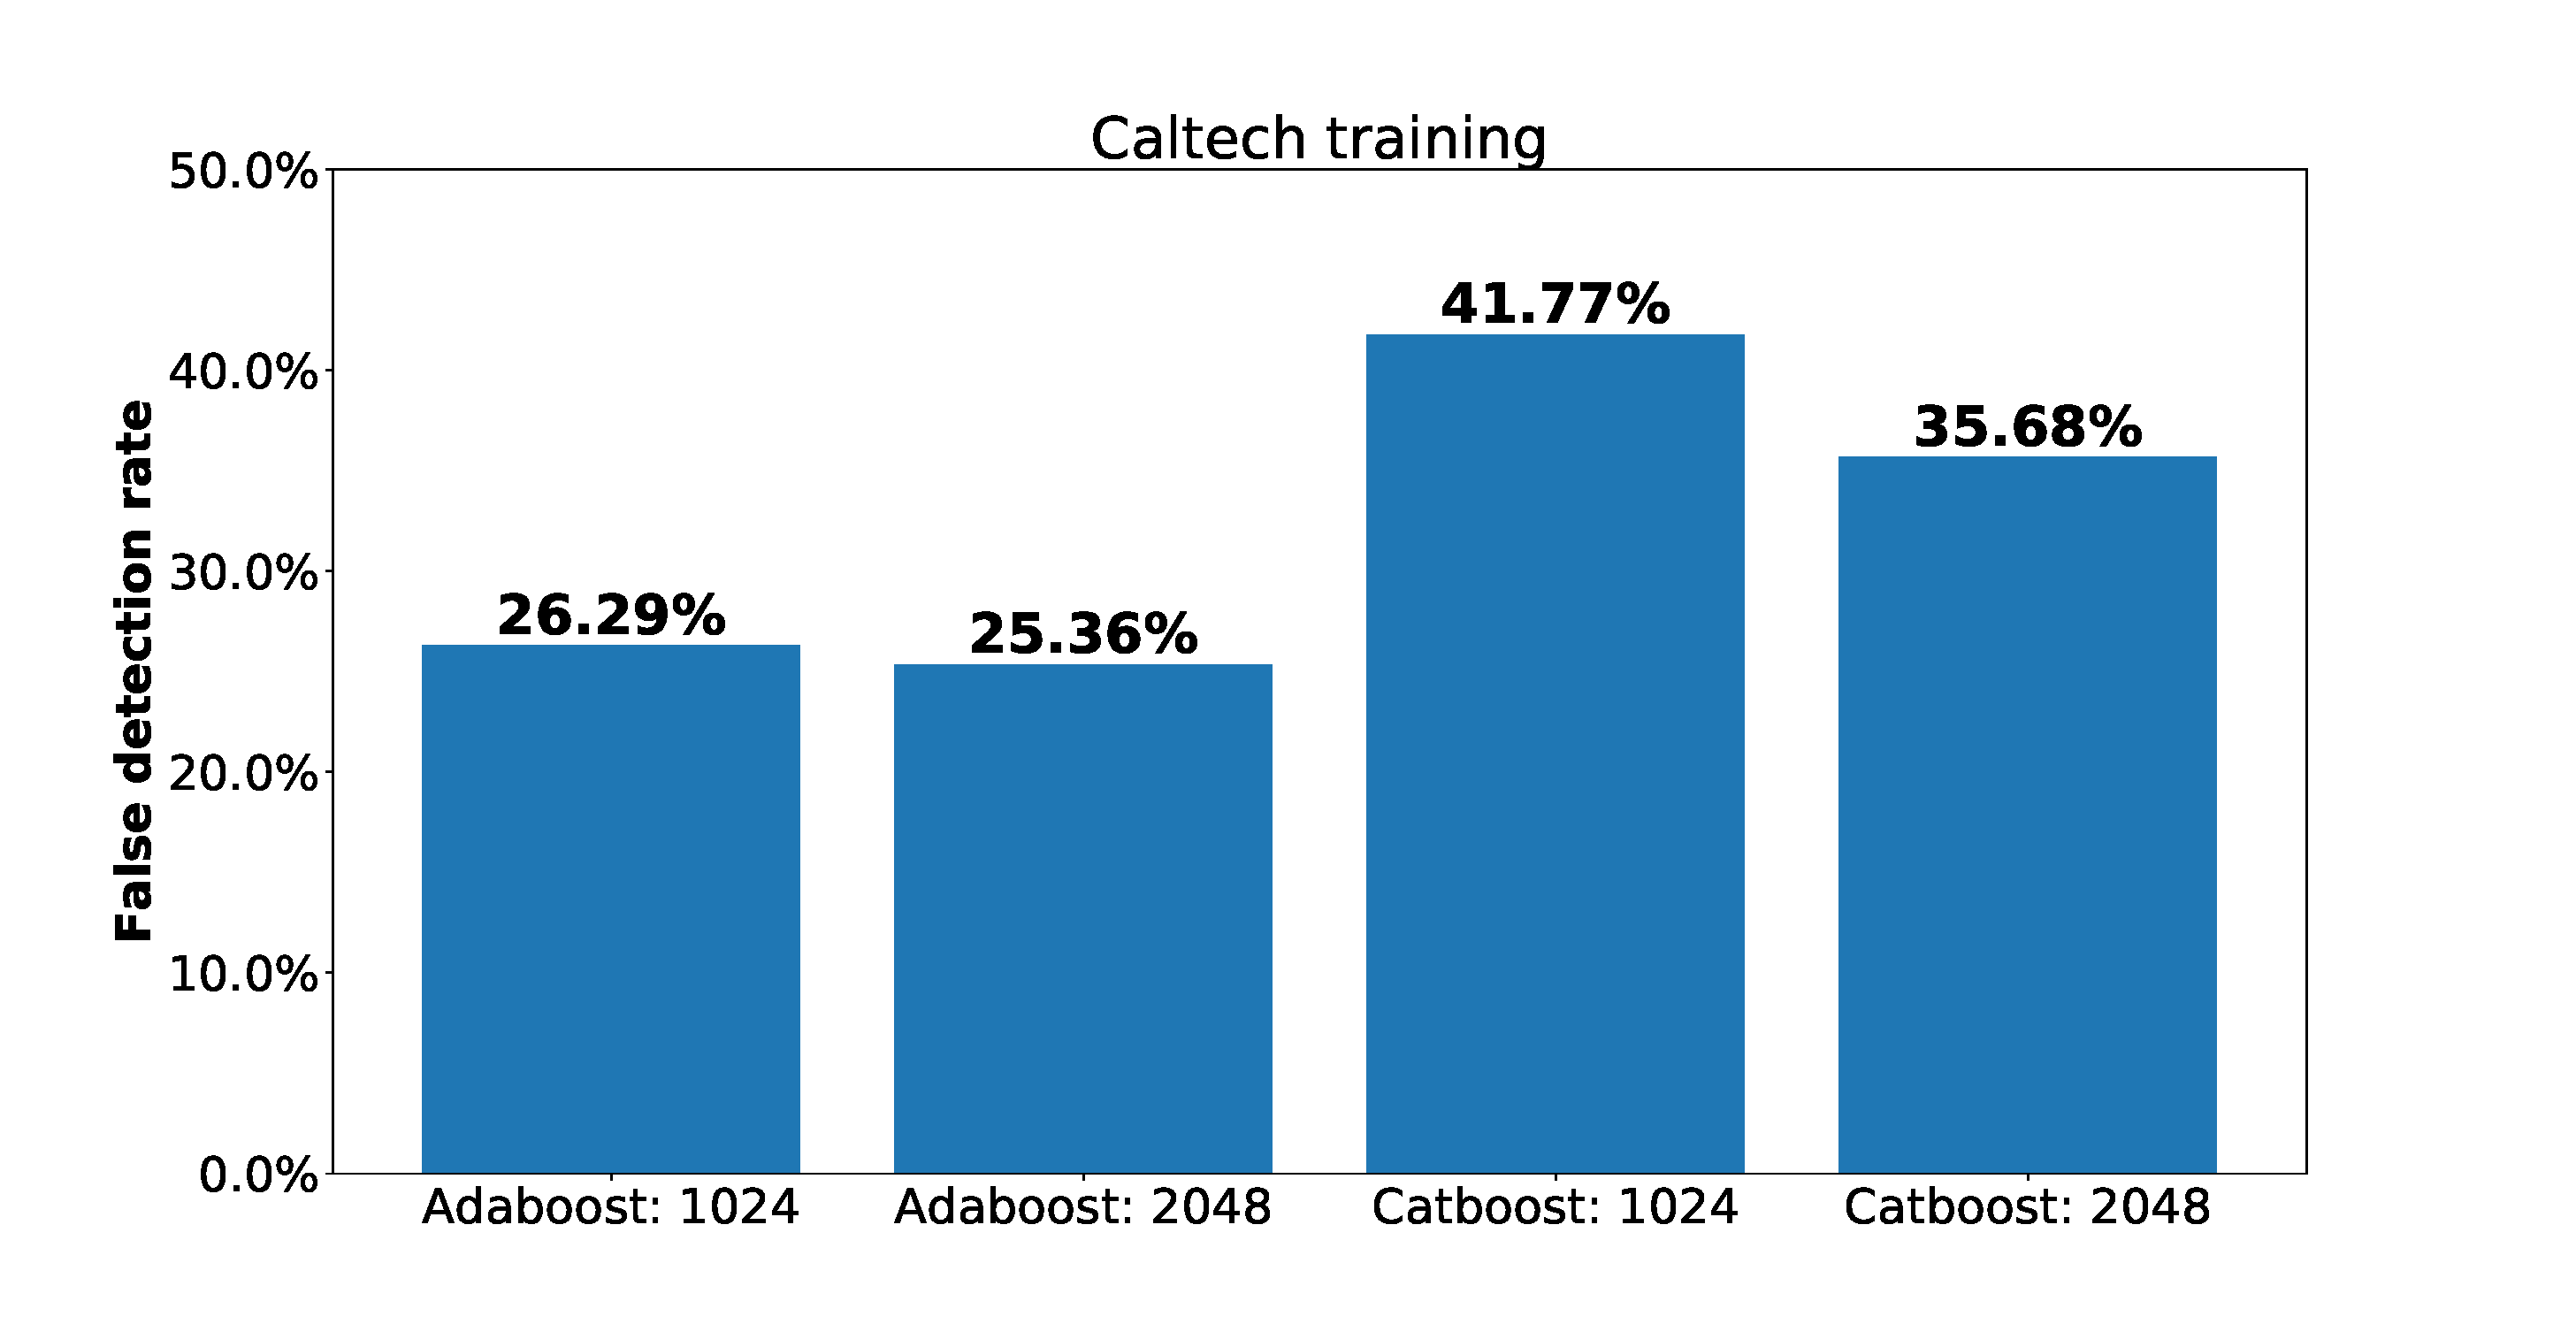
\includegraphics[width=1.1\linewidth]{figures/caltech_false_detection.eps}
          \caption{False detection rate para os clasificadores AdaBoost e CatBoost}
          \label{fig:sub3}
        \end{subfigure}
        \begin{subfigure}{.475\textwidth}
          \centering
          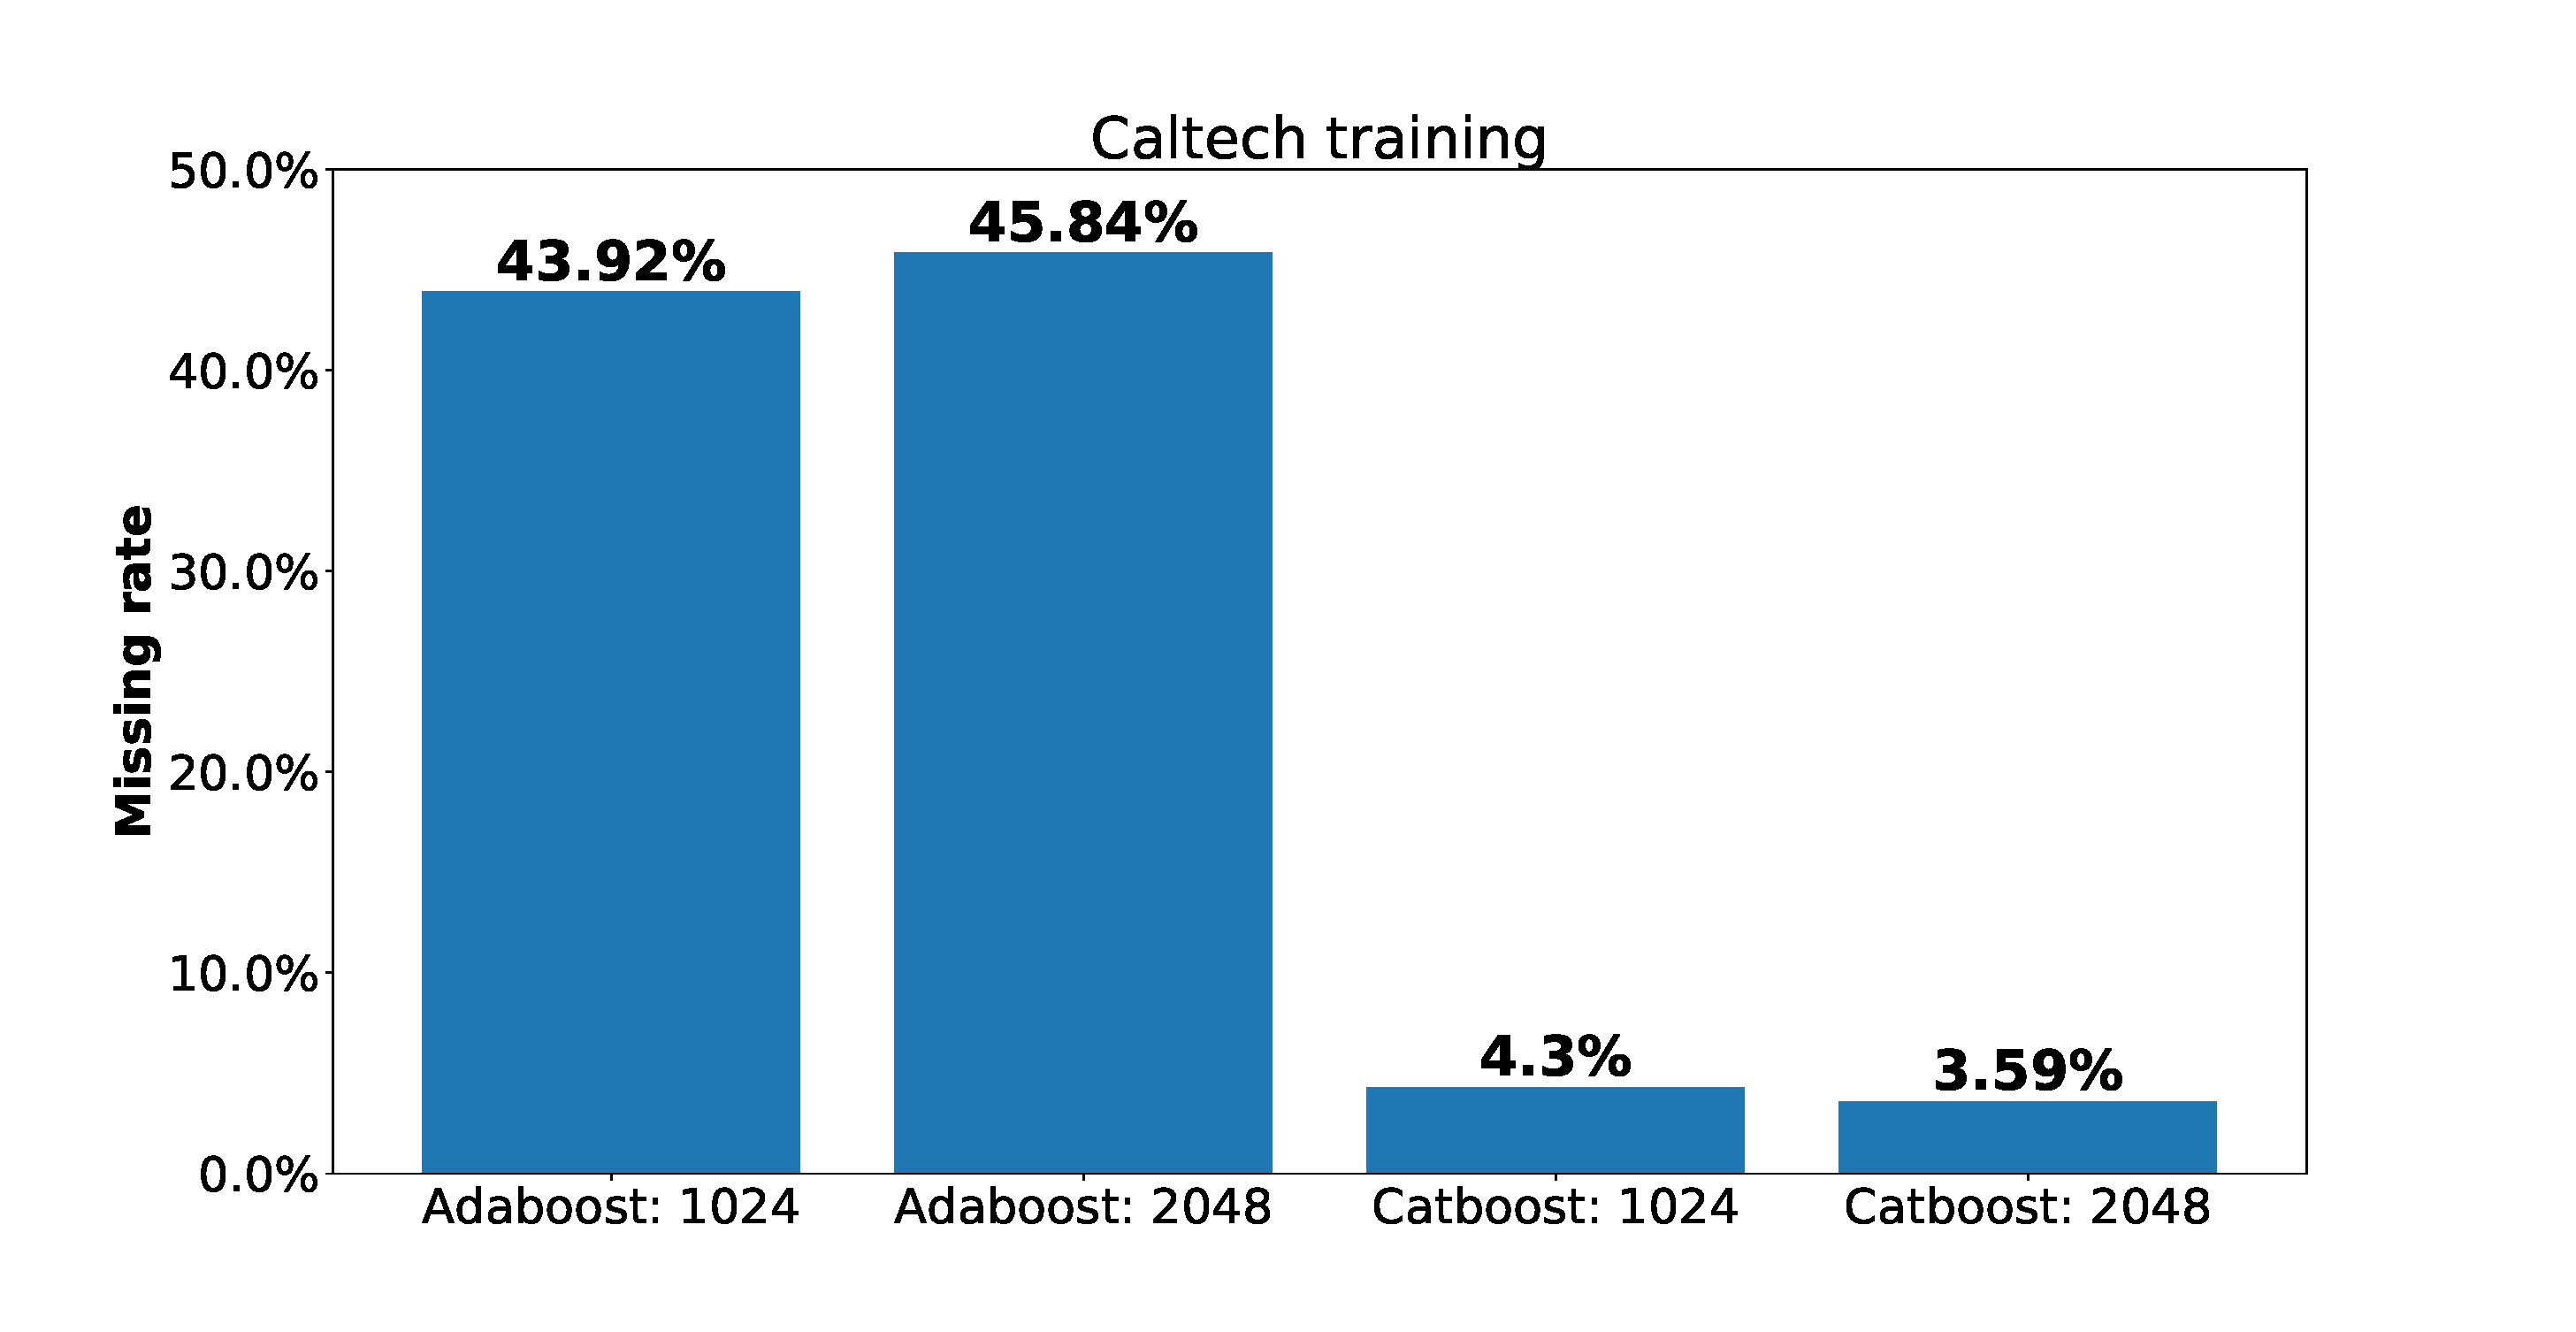
\includegraphics[width=1.1\linewidth]{figures/caltech_missing_rate.eps}
          \caption{Missing rate para os clasificadores AdaBoost e CatBoost}
          \label{fig:sub4}
        \end{subfigure}
        \caption{Resultados obtidos no adestramento có dataset INRIA \ref{fig:sub1} \ref{fig:sub2} e có dataset Caltech \ref{fig:sub3} \ref{fig:sub4}. En ámbolos casos móstrase ademais a evolución entre a ronda inicial (barras etiquetadas con 1024) e a de readestramento (barras etiquetdas con 2048).}
        \label{fig:results}
    \end{figure}
    
    Os resultados obtidos para o set de testeo mostránse na Fig. \ref{fig:results}. Nos dous casos (INRIA e Caltech) inclúese ademais do MR o FR para que se poida apreciar mellor a diferencia entre os resultados nos dous datasets. Os resultados correspondentes á ronda inicial son aqueles etiquetados con 1024 (nº de árbores de decisión) e os correspondentes á ronda de readestramento os de 2048. Según o dataset apréciase que:
    \begin{enumerate}
        \item No caso de INRIA os resultados para CatBoost son mellores que no caso de AdaBoost, chegando a baixar dun 12.32\% a un 8.37\% no MR. No caso do FR obsérvase que o seu valor é baixo (3.29\% como min.) pero para poder comparalo cos resultados do paper \cite{zhang} sería todavía necesario baixalo a uns valores <1\%. Isto é porque, nunha imaxe, o clasificador explicado na sección \ref{training} pode chegar a procesar máis de 60000 subimaxes e, con un FR de 3.29\%, só con que 1000 subimaxes sexan positivas isto supón ter ata 32.9 falsos positivos por imaxe (FPPI). Non obstante, para os valores obtidos en \cite{zhang} fálase duns 0.1 FPPI, o que demostra o lonxe que están estes resultados do pretendido.
        \par En canto á mellora nos resultados en MR de CatBoost respecto a AdaBoost, esta é coherente coa mellora demostrada polos seus creadores\cite{CatBoost}.
        \item En Caltech os resultados xa son máis dispares, notándose a diferencia de esixencia entre os datasets. Neste caso problabemente o que máis condiciona os resultados é a falta de máis rondas de readestramento engadindo negativos fortes. Isto apréciase no elevado valor en tódolos casos do FR (baixando a un mínimo duns 25.36\%). No MR, a diferencia presente entre ámbolos clasificadores explícase con que no caso de CatBoost consegue reducilo a costa de aumentar considerabelmente o FR, é dicir, deixando pasar máis falsos positivos.
        
    \end{enumerate}
        \begin{table}[t]
    \centering
        \begin{tabular}{c | c | c | c}
        Factor de escala & Núm. reescalados & paso xanela deslizante & Tempo \\ \hline
        1.33 & 6 & 60 px & 21.35 s \\ 
        1.09 & 6 & 60 px & 41.48 s \\ 
        1.33 & 10 & 60 px & 22 s \\ 
        1.09 & 10 & 60 px & 49.18 s \\
        1.33 & 3 & 6 px & 1714.82 s \\ 
        1.33 & 6 & 6 px & 1997.82 s \\ 
        1.09 & 6 & 6 px & 3479.2 s \\
        \end{tabular}
        \caption {Tempo de inferencia para o clasificador \textbf{CatBoost} para unha imaxe de 1024$\times$605 píxels en función do factor de escala para a imaxe, o número de reescalados e o tamaño do movemento en píxels da xanela deslizante ao percorrer a imaxe de entrada. Para facerse unha idea, no caso que máis tarda o clasificador está procesando un total de \textbf{65169 subimaxes}.}
        \label{tab:CatBoostTime} 
    \end{table}
    \begin{table}[t]
    \centering
        \begin{tabular}{c | c | c | c}
        Factor de escala & Núm. reescalados & paso xanela deslizante & Tempo \\ \hline
        1.33 & 6 & 60 px & 62.97 s \\ 
        1.09 & 6 & 60 px & 115.32 s \\ 
        1.33 & 10 & 60 px & 64.30 s \\ 
        1.09 & 10 & 60 px & 145.56 s \\
        1.33 & 3 & 6 px & 4633.17 s \\ 
        1.33 & 6 & 6 px & 5812.42 s \\ 
        1.09 & 6 & 6 px & 10156.83 s \\
        \end{tabular}
        \caption {Tempo de inferencia para o clasificador \textbf{AdaBoost} para unha imaxe de 1024$\times$605 píxels en función do factor de escala para a imaxe, o número de reescalados e o tamaño do movemento en píxels da xanela deslizante ao percorrer a imaxe de entrada.}
        \label{tab:AdaBoostTime} 
    \end{table}
    \par En canto ao tempo de inferencia do clasificador, empregouse o detector descrito na sección \ref{training}.
    \par Nel, a imaxe orixinal é reescalada varias veces aplicando un factor de escala e empregando un NMS (Non Maximum Suppression) para en caso de aparecer varias deteccións que se solapen, que só conten como unha.
    \par Nos cadros \ref{tab:CatBoostTime} e \ref{tab:AdaBoostTime} amósase o tempo que tarda o detector en procesar toda unha imaxe de $1024\times605$ píxels empregando un único proceso (sen utilizar concurrencia), variando certos parámetros como son o factor de escala, número de reescalados e a cantidade de píxels que se move a xanela cada vez que procesa unha subimaxe.
    \par No caso de utilizar concurrencia, no PC empregado para este proxecto os tempo podíanse reducir nun factor de 1/12 (número de núcleos do PC). Non obstante, aínda usando isto, os tempos están moi lonxe de podelos utilizar para tempo real, tendo que reducilos a, polo menos, 50ms (20Hz ou 20fps) por imaxe.
    \par No Anexo \ref{images} móstranse algunhas deteccións obtidas co clasificador Catboost sobre imaxes de testeo.
    
    %\begin{figure}
        %\centering
        %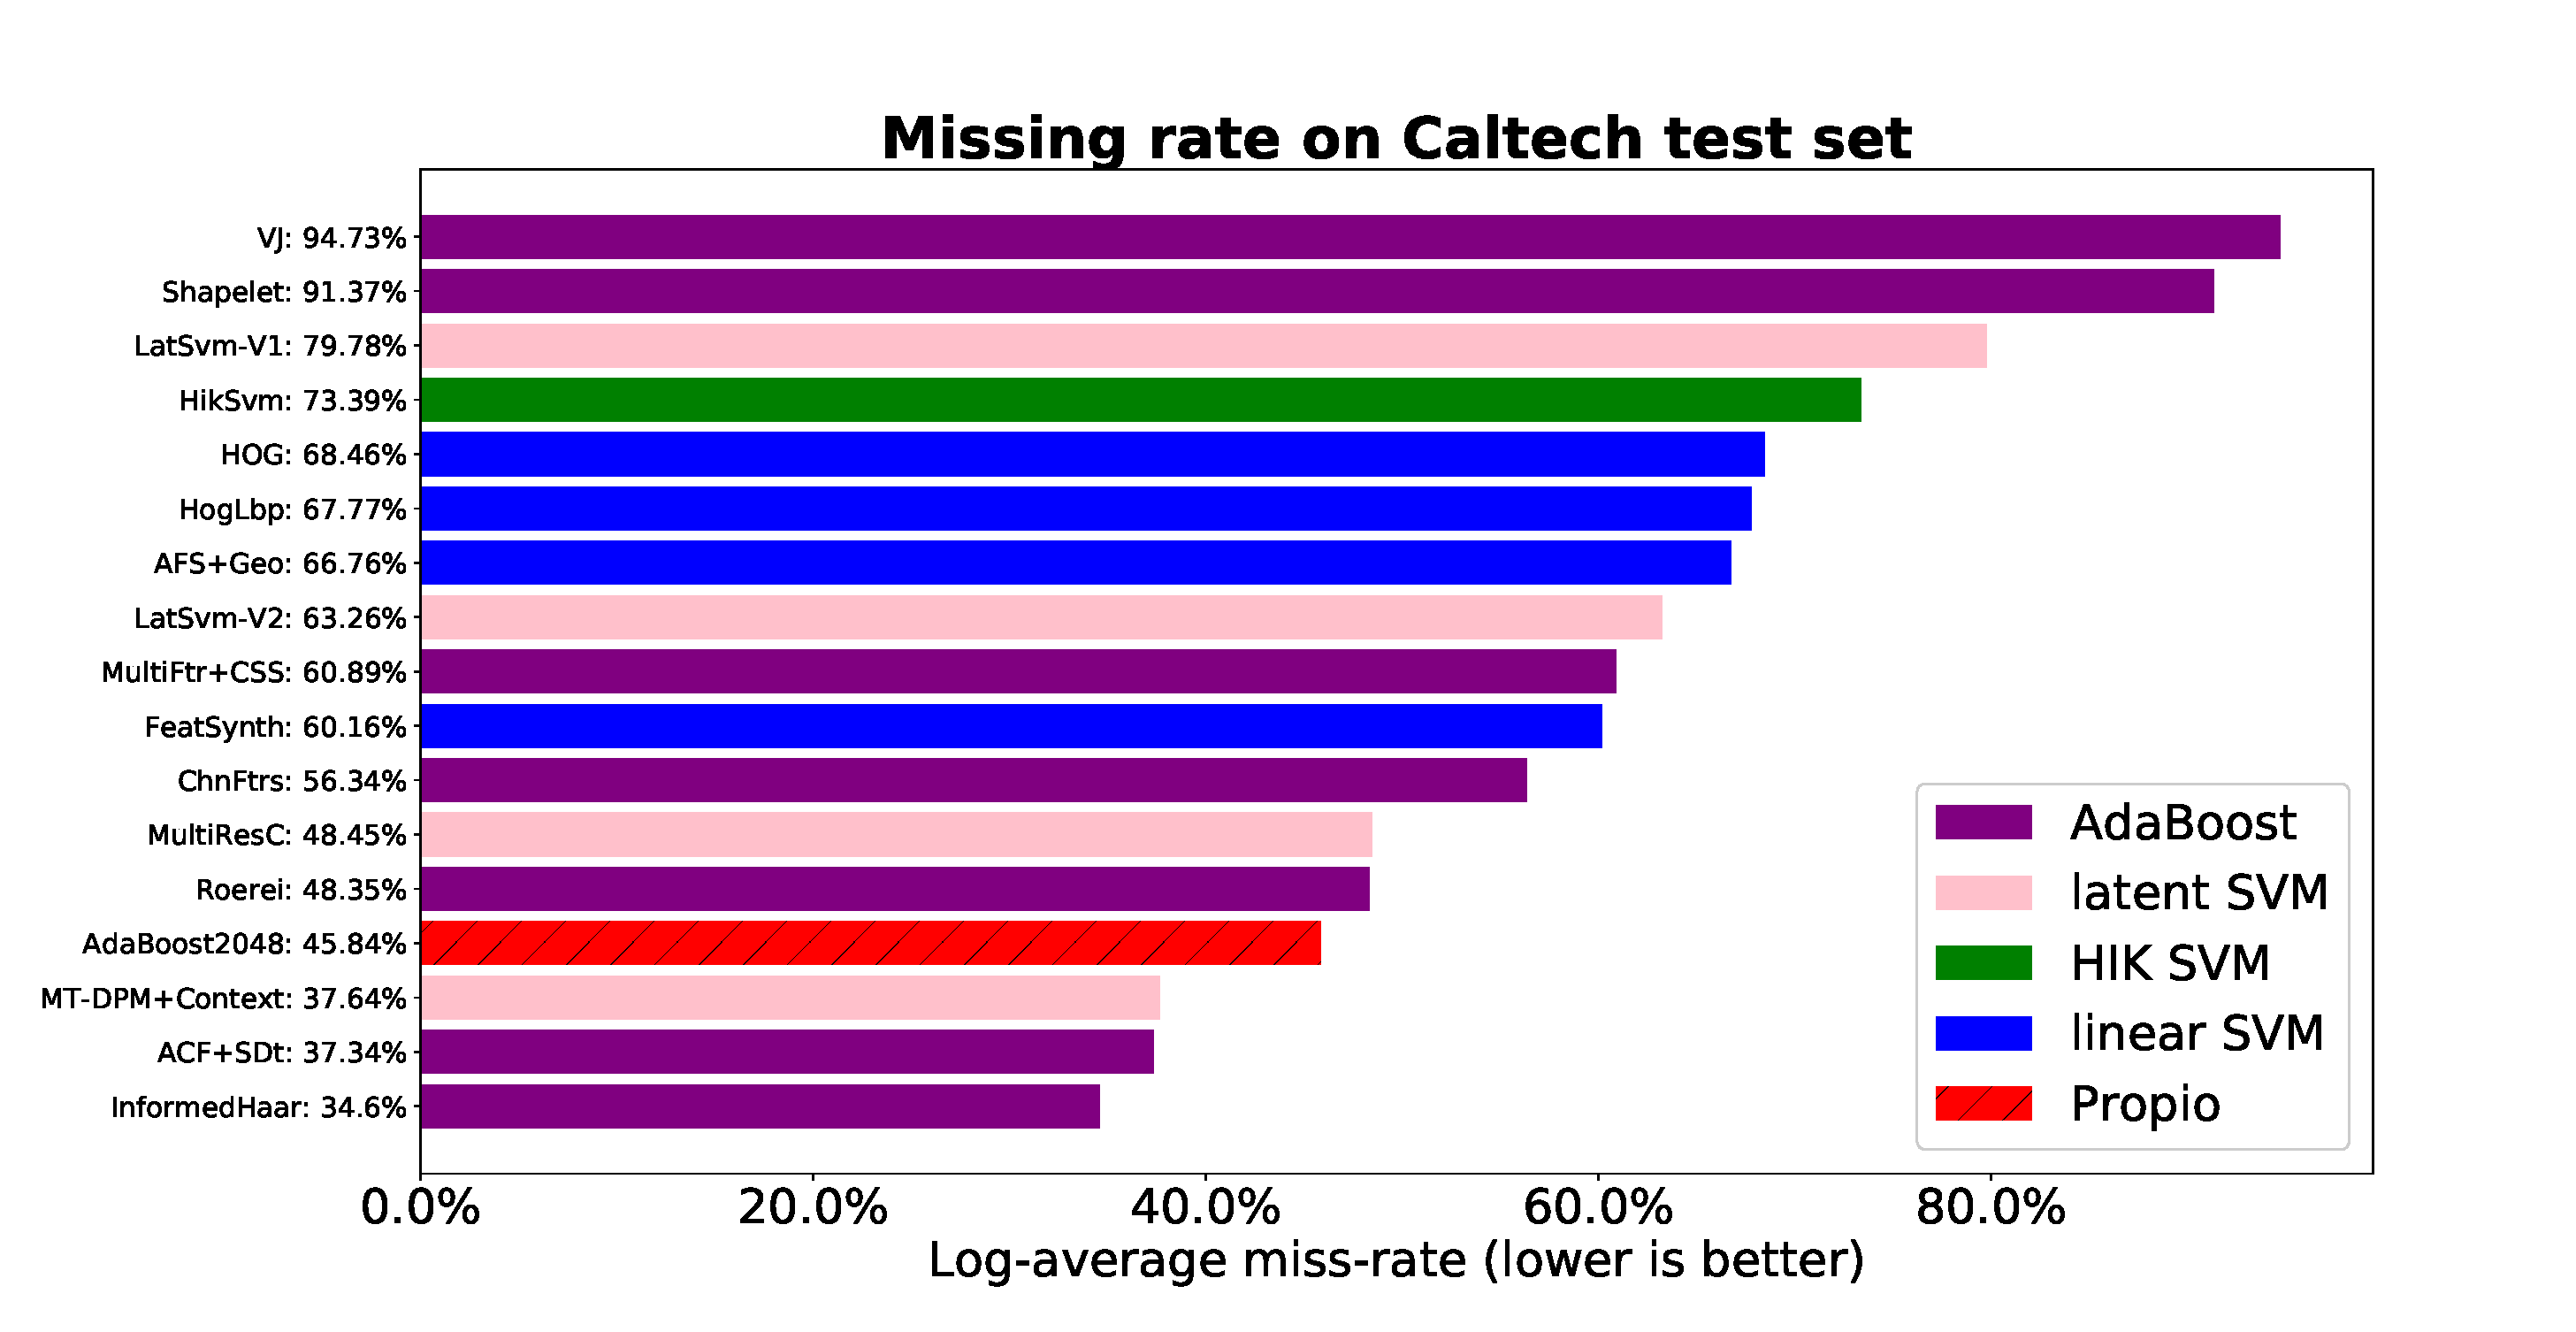
\includegraphics[height=200px]{figures/missing_rate_caltech_bars.eps}
        %\caption{Comparación do resultado en Caltech cos detectores de peóns no estado do arte actual. O resultado amosado é o de AdaBoost por ser o menor MR.}
        %\label{fig:caltechTest}
    %\end{figure}
    %\begin{figure}
        %\centering
        %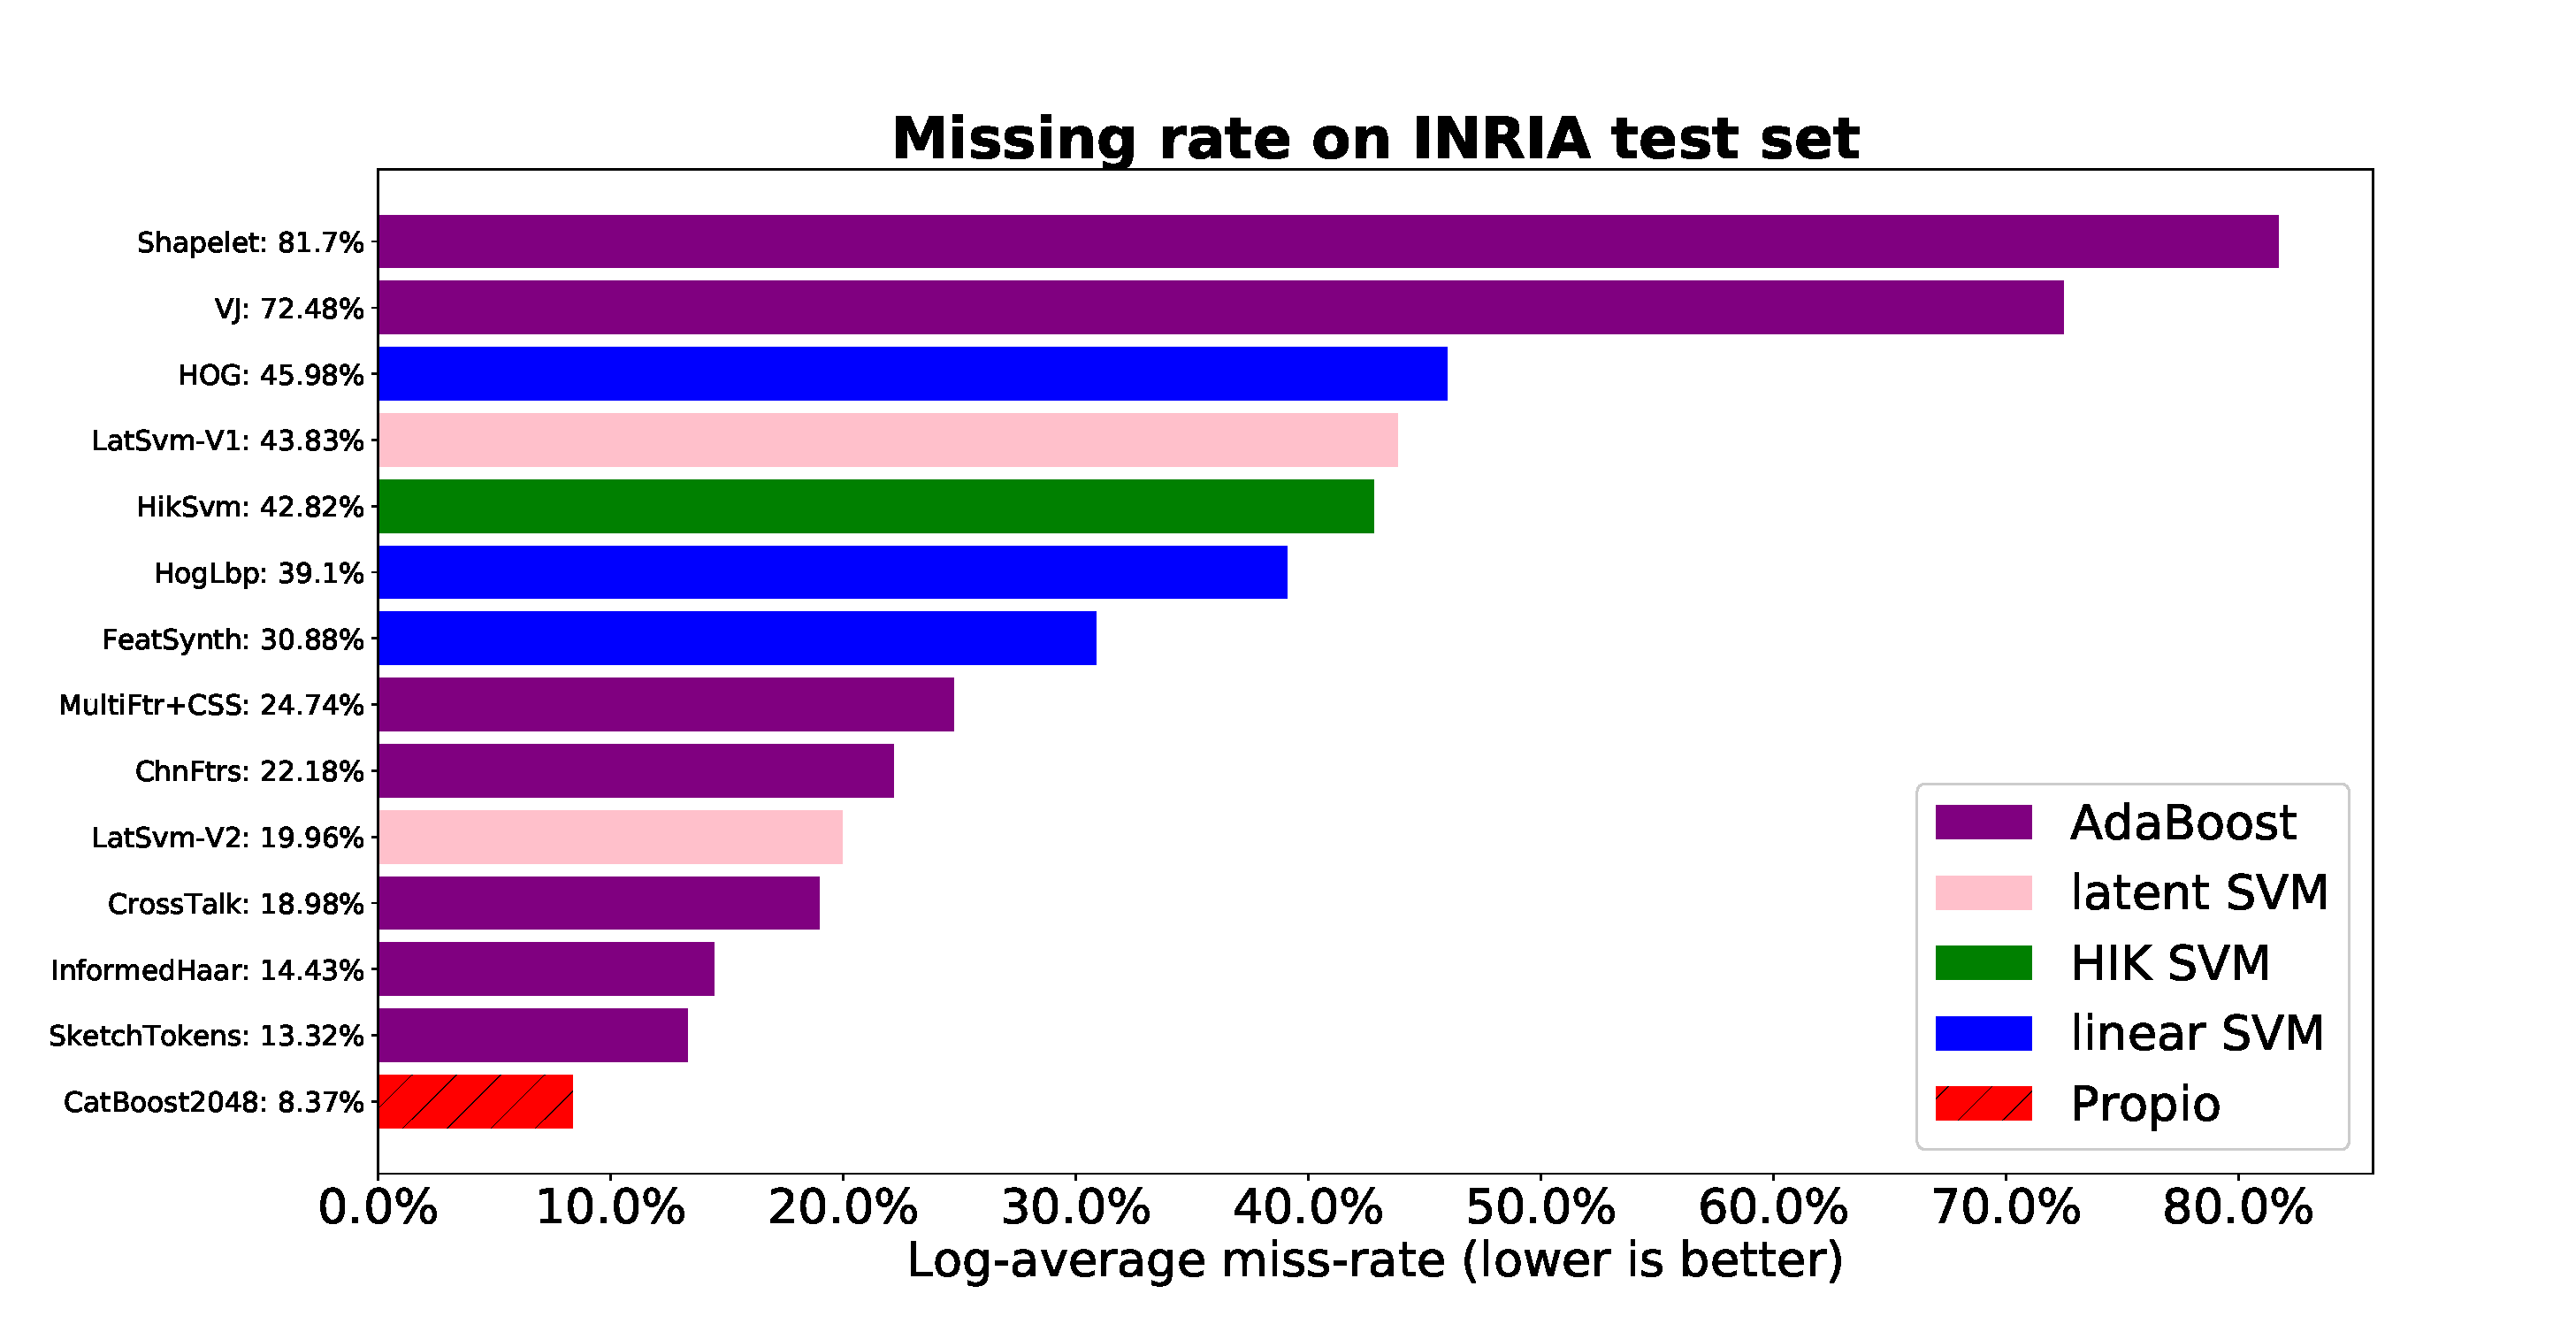
\includegraphics[height=200px]{figures/missing_rate_inria_bars.eps}
        %\caption{Comparación do resultado en INRIA cos detectores de peóns no %estado do arte actual. O resultado amosado é o de CatBoost.}
        %\label{fig:inriaTest}
    %\end{figure}
    
%--------- CONCLUSIÓN ---------
    \section{Conclusións}
    \par A pretensión deste proxecto era atinxir un clasificador cuns resultados razoábeis que permitise prescindir de ter que utilizar redes neurais profundas e que poidese funcionar en sistemas con baixos recursos. Para facerse unha idea, coa rede ResNet152\cite{he2016deep} de 152 capas na súa implementación en Python, para unha imaxe de 1024$\times$605 píxels (como a empregada nos cadros \ref{tab:CatBoostTime} e \ref{tab:AdaBoostTime}) o tempo de inferencia é de 4.607s (0.22fps) en media na CPU. Isto fai obvio que non é factíbel empregala para unha aplicación en tempo real.
    \par No caso dos clasificadores adestrados neste proxecto, o seu tempo de procesado é moito máis elevado polo que tampouco son válidos para ese tipo de aplicación.
    \par Para poder empregar os clasificadores en tempo real faise necesario implementalo noutra lenguaxe,  xa que Python pode chegar a ser 700 veces máis lento ca C++ e 70 veces máis que Matlab \cite{python}. Ademais á vista dos MR, é necesario aumentar o número de negativos fortes nos adestramentos para coseguir reducir o FR e, por conseguinte, o MR. É o caso de \cite{filtered} onde empregaron catro rondas de 10000 negativos fortes cada unha. Isto leva tamén á necesidade dunha gran cantidade de negativos, xa que extraer 10000 en cada ronda cada vez vólvese máis difícil ao funcionar moito mellor o clasificador.
    \par No caso presente, chegando a usar un conxunto de imaxes negativas de máis de 3000 non foi abondo para acadar os 10000 negativos para a segunda ronda de readestramento (recordando que os negativos fortes son do tamaño co que se adestrou o clasificador, polo que nunha imaxe negativa pode haber máis de 20 negativos fortes normalmente).
    \par Non obstante, aínda con estos resultados en canto a MR e FR os resultados con CatBoost son claramente moito mellores que no caso de AdaBoost, polo que poderíase acadar uns bos resultados levando a cabo as melloras citadas. 
    \par Ademais hoxe en día o dataset de INRIA consíderase insuficiente para conseguir bos resultados en case toda a documentación relacionada coa detección de peóns polo que tería máis sentido centrarse en Caltech, ou noutros datasets coma KITTI\cite{kitti}.
    \par Cabe destacar tamén que se empregaron tódalas características para facer as deteccións, o que supón calcular uns 10470 valores por imaxe, cando se poderían escoller aquelas con un mellor resultado, limitando os cálculos a por exemplo unhas 1000 características.
    \par Finalmente, engadindo certas técnicas habituais no procesado de imaxe, como é unha boa selección da zona de interese para a búsqueda de peóns ou facer a búsqueda unicamente nas escalas correspondentes coñecendo a distancia a que se encontran (facendo unha vista de paxaro), é posíbel acadar os resultados que se buscaban para este proxecto.
    
%---------REFERENCIAS---------
    \bibliographystyle{IEEEtran} 
    \bibliography{biblio/refs}
    
%---------ANEXOS---------
\appendix
    \section{Estado da arte}
    A detección de peóns é un problema amplamente investigado nos últimos 16 anos, sobre todo debido a tódalas súas posíbeis implicacións en distintos ámbitos como son a seguridade, ou a automoción. Dende os seus inicios no 2005 cando o primeiro detector por Viola e Jones empezou a funcionar\cite{viola2005detecting} ata a actualidade, fixéronse grandes avances. Moitos dos últimos papers e investigacións introducen novos métodos que presentan mellores resultados. Hoxe en día pódese dicir que os métodos máis empregados e investigados clasifícanse en dous tipos\cite{zhang2017towards}: ICF (Integral Channel Feature detector) e CNN(Convolutional Neural Network) para detección de peóns.
    
    \begin{itemize}
        \item \textbf{Detectores ICF}. Os detectores ICF foron propostos por \cite{dollar2014fast}\cite{dollar2009integral}, onde se demostrou que a orientación dos gradientes e as características de cor dunha imaxe (HOG+LUV), empregadas para mellorar árbores de decisión, eran máis efectivas e superaban facilmente os detectores previos. Para reducir os costes computacionais, algúns traballos propuxeron estudar unha aproximación ao cálculo das características mediante diferentes escalas e xanelas veciñas\cite{dollar2012crosstalk}. Para máis velocidade incluso propúxose un adestramento con varios modelos a diferentes escalas para evitar ter que reescalar a imaxe en tempo de procesado\cite{benenson2012pedestrian}.
        \par Non obstante, a maior parte dos esforzos foron dirixidos a obter os detectores con mellor rendemento\cite{benenson2013seeking}\cite{daniel2016semantic}\cite{nam2014local}\cite{paisitkriangkrai2014strengthening}\cite{zhang}\cite{zhang2015exploring}\cite{filtered}, onde se atopou que o que máis lle afecta é o tipo de filtros empregado. Algún exemplo dos anteriormente citados poden ser: \textit{SquareChntrs}\cite{benenson2014ten} que utiliza filtros cuadráticos promediados; \textit{InformedHaar}\cite{zhang} que básase en utilizar información da forma do corpo do peón; \textit{LDCF}\cite{nam2014local} que emprega autovectores que proveñen de análises linais discriminativas sobre imaxes naturais; \textit{RotatedFilters} que é unha versión simplificada dos \textit{LDCF}\cite{zhang2016far}; \textit{Checkerboards}\cite{filtered} que utiliza un conxunto de filtros  que inclúen detectores de gradiente vertical e horizontal e patróns tipo xadrez. Pódense apreciar algúns exemplos de posíbeis filtros na Fig. \ref{fig:filters}.
        \par Como resumo, os detectores ICF acadan uns resultados moi competitivos cunha complexidade computacional baixa; non obstante, hay que ter en conta tamén as súas desventaxes. A creación manual de características deseñadas intuitivamente basadas en, por exemplo, a forma do corpo, limitan o funcionamento do detector facendo máis posíbel a confusión con obxectos que se parezan na súa forma. Ademais, as árbores de decisións son máis rápidas a hora de testear, pero son máis sensíbeis ao ruido nas anotacións durante o adestramento.
        \item\textbf{Detectores basados en CNN}. As redes neurais convolucionais (CNN) acadaron moi bos resultados tanto en clasificación coma en detección en datasets coma ImageNet\cite{krizhevsky2012imagenet}, Pascal ou MS COCO. Non foi ata estes últimos anos que empezáronse a aplicar tamén en detección de peóns.
        \par A maior partes das CNN confían en outros métodos para a extracción das características, excepto no caso de \textit{ConvNet}\cite{sermanet2013pedestrian}, que emprega directamente a rede sobre a imaxe mediante unha xanela deslizante. \textit{DPM}\cite{felzenszwalb2009object} e \textit{HOG/linSVM}\cite{inria} foron os primeiros métodos en xurdir, mentres os detectores ICF íanse facendo cada vez máis populares. Posteriormente descubriuse que os ICF poden ser utilizados como candidatos moi eficaces para mellorar a precisión das CNN\cite{angelova2015real}\cite{hosang2015taking}.
        \par Recentemente, os detectores basados en CNN están tendendo a utilizar redes profundas (deep learning) como son \textit{AlexNet}\cite{krizhevsky2012imagenet}, \textit{GoogLeNet}\cite{szegedy2015going} e \textit{VGG}\cite{simonyan2014very}. Estas redes son capaces de facer deteccións de alta fiabilidade sen ter que depender de métodos externos. Non obstante este aumento da calidade e fiabilidade das deteccións ten un prezo: o aumento do custo computacional e a necesidade dunha mayor cantidade de datos para o adestramento. Ademais, xeralmente este tipo de redes teñen problemas para producir deteccións ben aliñadas, especialmente para obxectos pequenos.
    \end{itemize}
    
    \par En canto aos sets de imaxes utilizados para a evaluación e adestramento dos clasificadores, xurdiron varios diferentes ao longo da última década. INRIA\cite{inria}, ETH\cite{ess2008mobile} e TUD-Brussels\cite{wojek2009multi} foron os primeiros en aparecer e en tentar xuntar un número de imaxes significativo para facer investigacións referentes á detección de peóns. Hoxe en día Catech-USA\cite{caltech} e KITTI\cite{kitti} convertéronse nos máis populares debido a súa gran cantidade de información e a que son máis desafiantes que os anteriormente citados. Ambos datasets consisten en imaxes grabadas dende un coche a través dunha gran cidade, sendo para cada caso:
    \begin{itemize}
        \item Caltech-USA. Este dateset consiste en 2.5 horas de vídeos grabados a 30Hz dende un vehículo a través das rúas de Los Angeles, USA. Nos vídeos están anotados un total de 350k obxectos dos cales en torno a 2300 son peóns. O seu set de testeo consiste nun conxunto de 4024 frames. Habitualmente, para extraer as imaxes deste dataset utilízase unha de cada 30 imaxes do vídeo para evitar redundancia.
        \item KITTI. O dataset de KITTI foi capturado tamén a bordo dun vehículo que conducía a través da vila de Karlsruhe, Alemania, recollendo tanto zonas ruraris coma de autovía. Debido a que o set de testeo de KITTI non é público, normalmente sepárase o set de adestramento en dúas partes, empregando unha para testeo e outra para o adestramento propiamente dito.
    \end{itemize}
    \par Para a comparación, pódese ver o cadro \ref{tab:datasetTab}, onde se amosa que Caltech-USA e KITTI sobrepasan por moito en termos de volume a outros datasets.
    \begin{table}[t]
    \centering
        \begin{tabular}{c c c c c}
        \hline
        Dataset & Captura da imaxe & Imaxe en cor & Nº de imaxes & Nº de peóns \\ \hline
        Caltech-USA & móbil & Si & 122k & 155k \\ 
        KITTI & móbil & Si & 7518 & - \\  
        INRIA & estática & Si & 288 & 566 \\  
        ETH & móbil & Si & 1804 & 12k \\ 
        TUD-Brussels & móbil & Si & 508 & 1498 \\
        Daimler & móbil & Non & 21.8k & 56.5k \\
        \end{tabular}
        \caption {Comparación en canto a volume de datos entre distintos datasets (unicamente en referencia aos sets de testeo).}
        \label{tab:datasetTab} 
    \end{table}
    \begin{figure}[ht]
        \centering
        \begin{subfigure}{.5\textwidth}
          \centering
          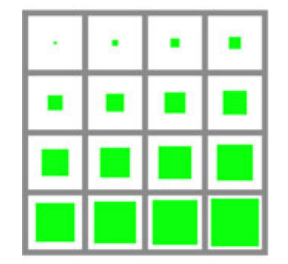
\includegraphics[width=.4\linewidth]{figures/SquaresChntrs.PNG}
          \caption{Exemplo de filtros SquaresChntrs\cite{benenson2014ten}}
          \label{fig:squares}
        \end{subfigure}%
        \begin{subfigure}{.5\textwidth}
          \centering
          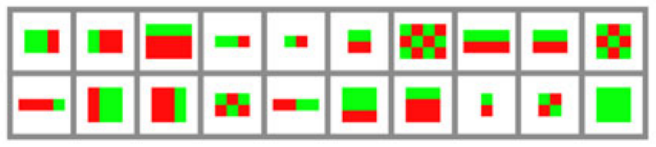
\includegraphics[width=.6\linewidth]{figures/Checkerboards.PNG}
          \caption{Exemplo de filtros Chekerboards\cite{filtered}}
          \label{fig:checkers}
        \end{subfigure}
        \caption{Comparación entre filtros de dous detectores ICF.}
        \label{fig:filters}
    \end{figure}
    
    
    %\section{Glosario}\label{glossary}
    \section{Tecnoloxías empregadas}
    \begin{enumerate}
        \item \textbf{AdaBoost (\textit{Adaptive Boosting)}}\cite{freund1997decision}. É un meta-algoritmo de aprendizaxe automática, proposto por Yoav Freund e Robert Schapire, que se emprega en conxunto con outros algoritmos para mellorar os resultados finais.
        \par O termo \textit{boosting} fai referencia a un tipo de algoritmos onde a finalidade é encontrar unha hipótese forte a partir de empregar hipóteses simples e febles. \textit{Adaptive} fai referencia a que propón adestrar unha serie de clasificadores débiles de maneira iterativa,  de forma que cada novo clasificador (\textit{weak learner}) só se enfoque nos datos que foron erroneamente clasificados polo seu predecesor, conseguindo que o algoritmo final se adapte e obteña mellores resultados.
        \item \textbf{CatBoost}\cite{CatBoost}. CatBoost é un algortimo \textit{open source} deseñado para \textit{gradient boosting} empregando árbores de decisión. Foi creado por investigadores de Yandex e é empregada por outras empresas como Cloudflare ou o CERN. Algunhas das súas principais ventaxes son a súa mellora, respecto a outros algoritmos similares, na predicción de clases e o soporte para adestramento multi-GPU.
        \item \textbf{Dataset Caltech-USA}\cite{caltech}. Este dateset consiste en 2.5 horas de vídeos grabados a 30Hz dende un vehículo a través das rúas de Los Angeles, USA. Nos vídeos están anotados un total de 350k obxectos dos cales en torno a 2300 son peóns. O seu set de testeo consiste nun conxunto de 4024 frames. Habitualmente, para extraer as imaxes deste dataset utilízanse unha de cada 30 imaxes do vídeo para evitar redundancia.
        \item \textbf{Dataset INRIA}\cite{inria}. INRIA é un dos datasets de peóns máis antigos e comparativamente cós actuais, é un dos máis reducidos. Consiste nunha serie de imaxes nas que aparecen peóns en distintos contextos, non só en cidade se non tamén en parques, nunha montaña, na praia, etc. Xeralemente, antes de que aparacesen os datasets máis recentes empregábase para o adestramento dos clasificadores polas súas anotacións das posicións dos peóns, que eran de gran calidade.
        \item \textbf{OpenCV}\cite{opencv_library}. OpenCV é unha libraría \textit{open source} centrada na visión artificial orixinalmente desenvolta por Intel. Actualmente (outubro de 2019) encóntrase na súa versión 4.1.2 e abarca máis de 2500 algoritmos de procesado de imaxe optimizados para o seu uso baixo unha licenza BSD. É unha libraría popular e de prestixio no seu campo (é empregada por Google, Intel, IBM, Honda...) e está dispoñíbel para tódalas plataformas (Windows, Linux, Android e Mac OS) e ten interfaces dispoñíbeis en Python, Java, C++ e MATLAB.
        \item \textbf{Scikit-learn}\cite{scikit-learn}. É unha libraría de \textit{machine learning} creada en 2007 para a lenguaxe de programación Python. Inclúe algoritmos de clasificiación, regresión e análise de grupos entre os cales están: \textit{Random Forest, AdaBoost, K-means e SVM}. Esta deseñada para traballar con outras librarías de Python como NumPy e SciPy. Está maiormente escrita en Python, aínda que algunhas partes escribíronse en Cython para mellorar o rendemento.
    \end{enumerate}
\newpage
\section{Deteccións en imaxes}\label{images}
        \begin{figure}[h]
        \centering
        \begin{subfigure}{.3\textwidth}
          \centering
            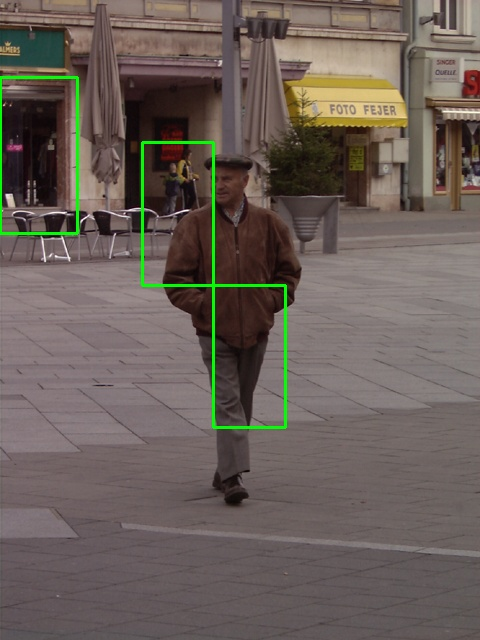
\includegraphics[width=0.8\linewidth]{figures/person1.jpg}
          \label{fig:person1}
        \end{subfigure}%
        \begin{subfigure}{.5\textwidth}
          \centering
          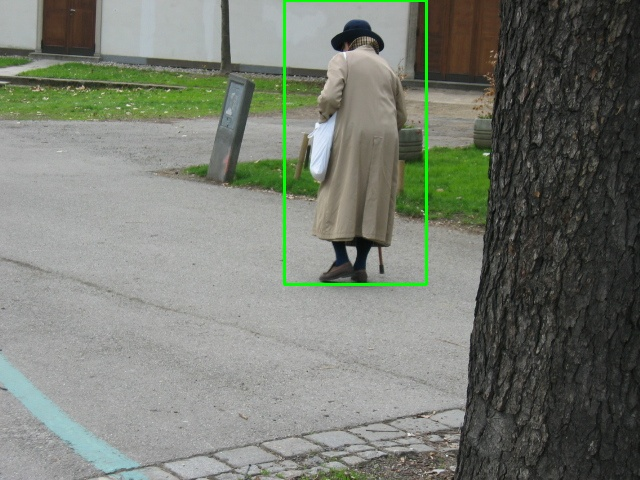
\includegraphics[width=0.8\linewidth]{figures/person2.jpg}
          \label{fig:person2}
        \end{subfigure}
        \begin{subfigure}{.5\textwidth}
          \centering
          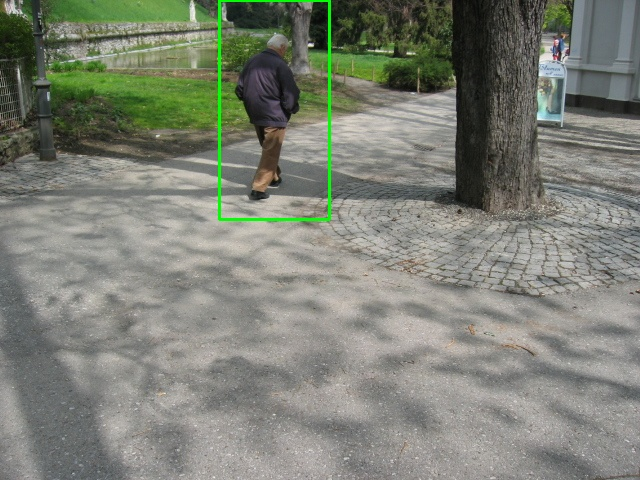
\includegraphics[width=0.8\linewidth]{figures/person3.jpg}
          \label{fig:person3}
        \end{subfigure}
        \begin{subfigure}{.3\textwidth}
          \centering
          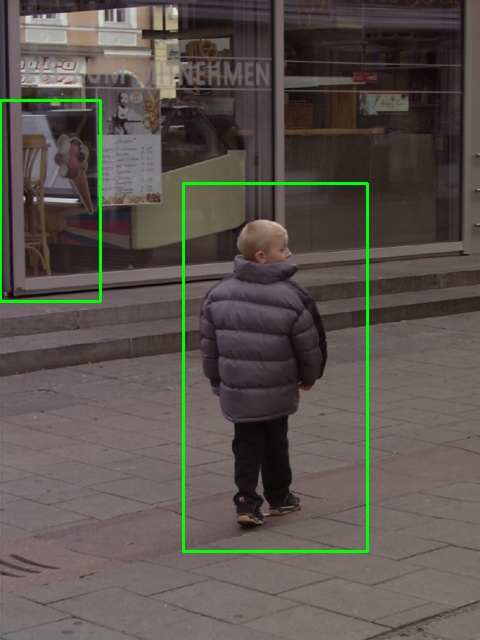
\includegraphics[width=0.8\linewidth]{figures/person4.jpg}
          \label{fig:person4}
        \end{subfigure}
        \begin{subfigure}{.3\textwidth}
          \centering
          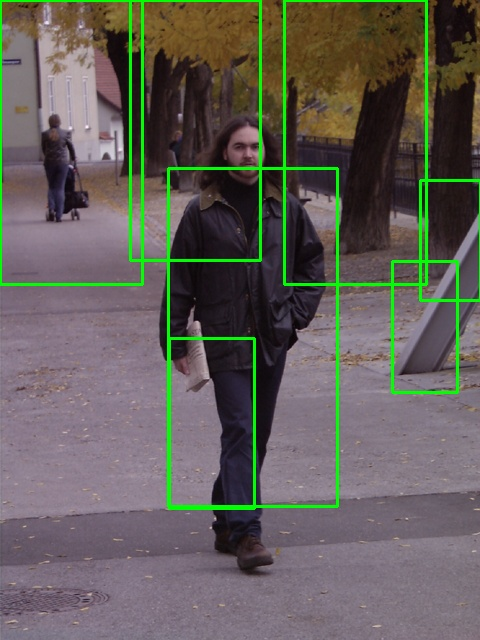
\includegraphics[width=0.8\linewidth]{figures/person5.jpg}
          \label{fig:person5}
        \end{subfigure}
        \begin{subfigure}{.3\textwidth}
          \centering
          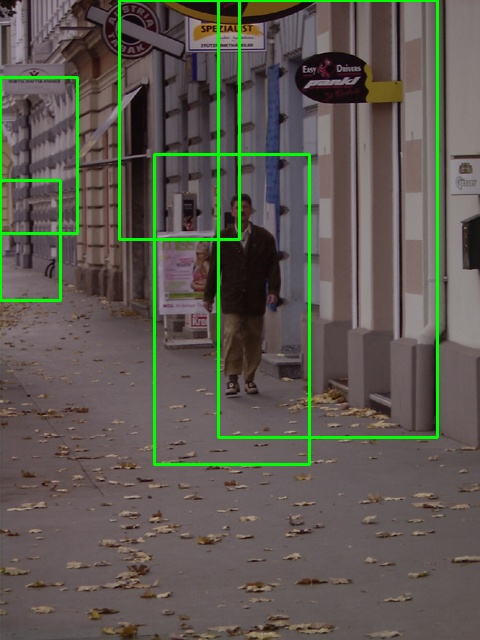
\includegraphics[width=0.8\linewidth]{figures/person6.jpg}
          \label{fig:person6}
        \end{subfigure}
        \begin{subfigure}{.3\textwidth}
          \centering
          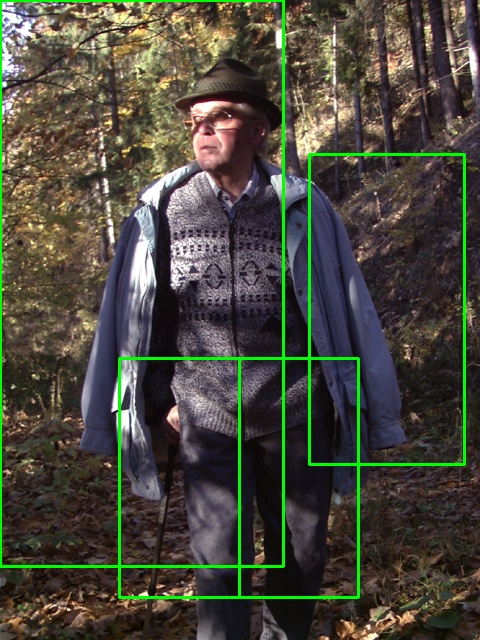
\includegraphics[width=0.8\linewidth]{figures/person8.jpg}
          \label{fig:person8}
        \end{subfigure}
        \caption{Deteccións obtidas empregando o clasificador Catboost sobre algunhas imaxes do set de testeo de INRIA. Recadrado en verde aparece aquelo que o clasificador detecta coma peón.}
        \label{fig:detections}
    \end{figure}
\end{document}
